\documentclass[11pt]{article}

\usepackage[margin=1in]{geometry}
\usepackage[T1]{fontenc}
\usepackage[utf8]{inputenc}
\usepackage{lmodern}
\usepackage{microtype}
\usepackage{amsmath,amssymb,mathtools}
\usepackage{booktabs}
\usepackage{graphicx}
\usepackage{siunitx}
\usepackage{pgfplots}
\usepackage{pgfplotstable}
\usepackage{tikz}
\usepackage{enumitem}
\usepackage{xcolor}
\usepackage{hyperref}
\usepackage{float}

\hypersetup{
  hidelinks,
  pdftitle={StanThrust Solver Notes},
  pdfauthor={StanThrust Project}
}

\pgfplotsset{compat=1.18}
\usetikzlibrary{arrows.meta,positioning,shapes.geometric,fit,backgrounds}
\sisetup{detect-all}

\definecolor{stanred}{HTML}{C51E35}
\definecolor{stanredbright}{HTML}{DE324A}
\definecolor{stancharcoal}{HTML}{171B21}
\definecolor{stanmuted}{HTML}{746B63}
\definecolor{stanfuel}{HTML}{D6A15D}
\definecolor{stanoxidizer}{HTML}{E05564}
\definecolor{stancooling}{HTML}{E5C46D}

\newcommand{\SampleFuel}{Ethanol}
\newcommand{\SampleFlowMode}{Refined quasi-1D solve}
\newcommand{\SampleOxidizer}{Liquid Oxygen}
\newcommand{\SampleMixtureRatio}{1.40}
\newcommand{\SampleTargetThrust}{250.0}
\newcommand{\SampleBurnTime}{12.00}
\newcommand{\SampleChamberLength}{51.6}
\newcommand{\SampleNozzleLength}{51.3}
\newcommand{\SampleThroatDiameter}{11.5}
\newcommand{\SampleExitDiameter}{20.6}
\newcommand{\SampleExpansionRatio}{3.219}
\newcommand{\SampleContourMethod}{MOC-informed bell contour}
\newcommand{\SampleReferenceConicalLength}{18.0}
\newcommand{\SampleBellLengthFraction}{1.000}
\newcommand{\SampleBellEntranceAngle}{23.30}
\newcommand{\SampleBellExitAngle}{3.03}
\newcommand{\SampleThroatEntryBlendRadius}{7.7}
\newcommand{\SampleThroatExitBlendRadius}{2.2}
\newcommand{\SampleInjectorOrificeCount}{24}
\newcommand{\SampleInjectorElementRing}{50.4}
\newcommand{\SampleChamberPressure}{1721.2}
\newcommand{\SampleThrust}{245.9}
\newcommand{\SampleIsp}{192.7}
\newcommand{\SampleCstar}{1373.7}
\newcommand{\SampleExitMach}{2.50}
\newcommand{\SampleGamma}{1.2083}
\newcommand{\SampleGasConstant}{391.3}
\newcommand{\SampleChamberTemperature}{3223.0}
\newcommand{\SampleThermoSource}{cantera-equilibrium-rocket\_mech\_equilibrium.yaml:rocket\_detailed}
\newcommand{\SampleNozzleEfficiency}{0.8821}
\newcommand{\SampleOverallNozzleEfficiency}{0.8821}
\newcommand{\SampleIterations}{6}
\newcommand{\SamplePressureFedFinalTankPressure}{693.2}
\newcommand{\SamplePressureFedFeedDrift}{55.10}
\newcommand{\SamplePumpFedFeedDrift}{0.00}


\newcommand{\clip}{\operatorname{clip}}
\newcommand{\mdot}{\dot{m}}
\newcommand{\mdotp}{\dot{m}_{p}}
\newcommand{\mdotf}{\dot{m}_{f}}
\newcommand{\mdoto}{\dot{m}_{ox}}
\newcommand{\Rey}{\operatorname{Re}}
\newcommand{\OF}{\left(\frac{O}{F}\right)}

\title{\textbf{StanThrust Solver Notes}\\\large Geometry, Feed-System, MOC, Viscous Flow, Thermal, and Structural Formulation}
\author{StanThrust Documentation Package}
\date{\today}

\begin{document}
\maketitle

\section{Purpose}
StanThrust is a liquid-engine sizing and analysis tool with a coupled design solver stack. The software takes a mission request or an as-built hardware definition, constructs a geometry bundle, solves the injector and feed hydraulics together with chamber mass balance, evaluates a burn-time feed transient, calls a Cantera thermochemistry provider, and then evaluates thrust, impulse, structural margins, and export geometry with a chamber/nozzle flow model. The software exposes fast preview, refined characteristic-net, and viscous quasi-one-dimensional modes. The final desktop solve uses the densest in-app station model so the saved state is based on the most detailed available calculation.

This report is written as an engineering methods note for the \emph{current StanThrust solver}. The goal is to show, in explicit algebraic form, how the program moves from a mission request to geometry, flow quantities, pressures, and performance values. The representative plots in this document come from the default packaged case:
\[
\text{fuel}=\text{\SampleFuel}, \qquad
\text{oxidizer}=\text{\SampleOxidizer}, \qquad
\OF=\SampleMixtureRatio, \qquad
F_{\text{target}}=\SI{\SampleTargetThrust}{N}, \qquad
t_b=\SI{\SampleBurnTime}{s}.
\]
The same solver histories used to generate the report figures are also exposed directly in the Qt desktop application through a dedicated plots tab, so the packaged UI and this document refer to the same transient, axial, and convergence data products.

When reading the report, each section can be interpreted in the same sequence used during preliminary engine sizing:
\begin{enumerate}[leftmargin=6mm]
\item start from the mission targets and packaging constraints;
\item convert those into geometry and propellant requirements;
\item check that the feed system can support the resulting chamber pressure;
\item evaluate how the feed state drifts across the burn;
\item evaluate the nozzle and chamber performance model;
\item compare the resulting scale against benchmark hardware.
\end{enumerate}

\section{Pipeline Overview}
\begin{figure}[H]
\centering
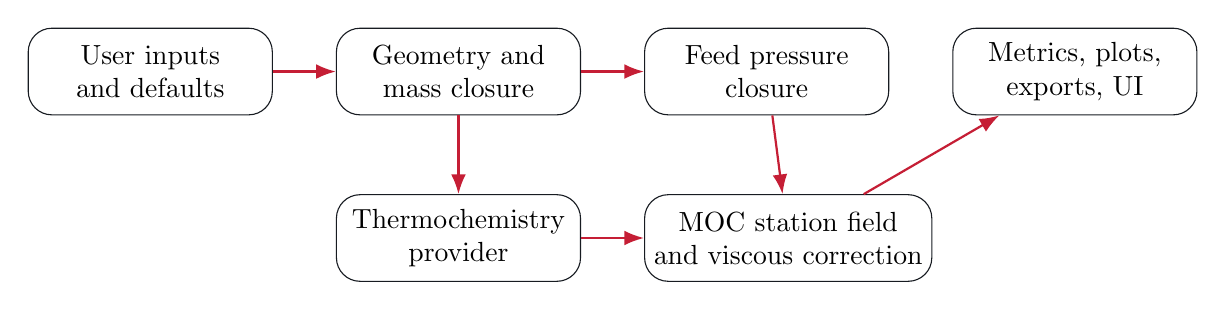
\begin{tikzpicture}[
  node distance=10mm and 8mm,
  box/.style={draw=stancharcoal, rounded corners=3mm, fill=white, minimum width=31mm, minimum height=11mm, align=center},
  line/.style={-{Latex[length=2.5mm]}, thick, draw=stanred}
]
\node[box] (ui) {User inputs\\and defaults};
\node[box, right=of ui] (geometry) {Geometry and\\mass closure};
\node[box, right=of geometry] (pressure) {Feed pressure\\closure};
\node[box, below=of geometry] (thermo) {Thermochemistry\\provider};
\node[box, right=of thermo] (combustion) {MOC station field\\and viscous correction};
\node[box, right=of pressure] (outputs) {Metrics, plots,\\exports, UI};

\draw[line] (ui) -- (geometry);
\draw[line] (geometry) -- (pressure);
\draw[line] (geometry) -- (thermo);
\draw[line] (pressure) -- (combustion);
\draw[line] (thermo) -- (combustion);
\draw[line] (combustion) -- (outputs);
\end{tikzpicture}
\caption{Current StanThrust solver flow.}
\end{figure}

The software is therefore a staged closure:
\begin{enumerate}[leftmargin=6mm]
\item normalize the input request;
\item generate a first-pass geometry and flow state;
\item enforce feed feasibility for either pump-fed or pressure-fed architecture;
\item obtain $(\gamma, R, T_c)$ from thermochemistry;
\item compute nozzle performance, mass flow, and predicted thrust;
\item evaluate heat transfer, material stress, redesign requirements, and uncertainty bounds.
\end{enumerate}

\section{Implementation Architecture}
The active Python package is rooted at \texttt{stanthrust/}. It keeps shared inputs and output contracts centralized while preserving separate files for physically distinct numerical models. This avoids duplicated constants without combining unrelated equations into one oversized module. The implementation map below lists paths relative to that package root.

\begin{table}[H]
\centering
\caption{Active StanThrust implementation map.}
\begin{tabular}{p{0.30\textwidth}p{0.61\textwidth}}
\toprule
Area & File and responsibility \\
\midrule
Inputs & \texttt{inputs.py}. Default state, selectable propellants and materials, objective weights, and numerical assumptions. \\
Design closure & \texttt{design\_model.py}. Mission normalization, chamber-pressure closure, component sizing, and solved geometry. \\
Flow solver & \texttt{combustion\_cfd\_solver.py}. Cantera coupling, MOC station fields, shock feedback, and final viscous correction. \\
Feed system & \texttt{feed\_pressure\_drop\_solver.py}. Pump-fed and pressure-fed transient loss and margin closure. \\
Nozzle physics & \texttt{moc\_nozzle\_solver.py}, \texttt{shock\_solver.py}. Characteristic-net geometry and Rankine-Hugoniot relations. \\
Thermal and stress & \texttt{heat\_transfer\_solver.py}, \texttt{structural\_material\_solver.py}. Wall temperature, stress, material ranking, and redesign checks. \\
Outputs & \texttt{uncertainty.py}, \texttt{exporter.py}. Provenance, uncertainty bands, project files, CSV data, and DXF profiles. \\
Desktop & \texttt{qt\_desktop.py}. Controls, progress, diagnostics, plots, and calculated-geometry rendering. \\
\bottomrule
\end{tabular}
\end{table}

The desktop application, documentation generator, and regression tests import these same modules. There is no separate documentation-only physics path. Experimental sensitivity code that was not connected to the final solve has been removed, so every solver method described in this report corresponds to an active application path.

\section{Symbols and Conventions}
\begin{table}[H]
\centering
\caption{Primary symbols used in the StanThrust formulation.}
\begin{tabular}{ll}
\toprule
Symbol & Meaning \\
\midrule
$F_{\text{target}}$ & user-requested thrust \\
$I_{\text{target}}$ & user-requested total impulse \\
$t_b$ & burn time \\
$P_c$ & chamber pressure \\
$A_c, A_t, A_e$ & chamber, throat, and exit area \\
$d_c, d_t, d_e$ & chamber, throat, and exit diameter \\
$L_c, L_n$ & chamber and nozzle length \\
$\gamma$ & ratio of specific heats from thermochemistry \\
$R$ & specific gas constant from thermochemistry \\
$T_c$ & chamber temperature from thermochemistry \\
$c^\star$ & characteristic velocity \\
$C_F$ & thrust coefficient \\
$\mdotp$ & total propellant mass flow \\
$\mdotf, \mdoto$ & fuel and oxidizer mass flow \\
$\varepsilon$ & expansion ratio $A_e/A_t$ \\
$t_w$ & wall thickness \\
\bottomrule
\end{tabular}
\end{table}

Whenever StanThrust constrains a value between lower and upper bounds, this report writes the operation as
\[
\clip(x,x_{\min},x_{\max})=\min\!\left(x_{\max},\max(x_{\min},x)\right).
\]

\section{Input Normalization and Scaling}
The initial sizing logic does not work directly on raw thrust and impulse. It first converts them into bounded nondimensional scaling factors:
\begin{equation}
S_F=\clip\!\left(\left(\frac{F_{\text{target}}}{250}\right)^{0.22},\,0.7,\,2.4\right)
\label{eq:thrust-scale}
\end{equation}
\begin{equation}
S_I=\clip\!\left(\left(\frac{I_{\text{target}}}{3000}\right)^{0.16},\,0.75,\,2.2\right)
\label{eq:impulse-scale}
\end{equation}
\begin{equation}
S_b=0.72+\frac{t_b}{28}
\label{eq:burn-factor}
\end{equation}
\begin{equation}
\beta_{\text{mix}}=\clip\!\left(\frac{\OF}{1+\OF},\,0.18,\,0.86\right).
\label{eq:mix-bias}
\end{equation}

Additional multipliers are derived from propellant catalog properties and user-selected architecture:
\begin{equation}
\phi_f = 1 + (0.62-\rho_f^\ast)\,0.42,
\qquad
\phi_{ox} = 1 + (0.68-\rho_{ox}^\ast)\,0.36
\label{eq:density-terms}
\end{equation}
where $\rho^\ast$ denotes the catalog density index rather than dimensional density.

The architecture and cooling modifiers are
\begin{equation}
\phi_{\text{blowdown}}=
\begin{cases}
1.0, & \text{pump-fed}\\
1.2, & \text{pressure-fed}
\end{cases}
\qquad
\phi_{\text{regen}}=
\begin{cases}
0.92, & \text{regen enabled}\\
1.0, & \text{otherwise}
\end{cases}
\qquad
\phi_{\text{film}}=
\begin{cases}
1.04, & \text{film cooling enabled}\\
1.0, & \text{otherwise}
\end{cases}
\label{eq:architecture-modifiers}
\end{equation}
and the propellant thermal modifier is
\begin{equation}
\phi_T = 1 + 0.12\,\tau_{ox} - 0.08\,\chi_f
\label{eq:thermal-modifier}
\end{equation}
with $\tau_{ox}$ the oxidizer thermal-severity index and $\chi_f$ the fuel cooling-affinity index from the internal propellant catalog.

\section{Geometry Closure}
\subsection{Tank, Chamber, and Nozzle Lengths}
The first-pass axial layout is generated from multiplicative closures. The fuel and oxidizer tank lengths are
\begin{equation}
L_{f,\text{tank}}
=
d_{\text{tank}}\,
\Pi_{\text{tank}}\,
S_b\,
S_I\,
\phi_f\,
\left(1.04-0.22\,\beta_{\text{mix}}\right)\,
\phi_{\text{blowdown}}
\label{eq:fuel-tank-length}
\end{equation}
\begin{equation}
L_{ox,\text{tank}}
=
d_{\text{tank}}\,
\Pi_{\text{tank}}\,
S_b\,
S_I\,
\phi_{ox}\,
\left(0.88+0.36\,\beta_{\text{mix}}\right)\,
\phi_{\text{blowdown}}
\label{eq:ox-tank-length}
\end{equation}
where $\Pi_{\text{tank}}$ is the packaging multiplier associated with the selected packaging bias.

The chamber barrel length is now sized from a characteristic-length target rather than only from a packaging multiplier. The chamber contraction ratio is
\begin{equation}
\varepsilon_c=\frac{A_c}{A_t}
\label{eq:chamber-contraction-ratio}
\end{equation}
and the target characteristic length is computed from propellant severity, injector family, thrust scale, packaging preference, and cooling state:
\begin{equation}
L^\star_{\text{target}}
=
\clip\!\left(
\left[
980
+260\tau_{ox}
-115\chi_f
+180\left|\beta_{\text{mix}}-0.5\right|
+45(S_F-1)
\right]\phi_{\text{inj}}\phi_{\text{pkg}}\phi_{\text{cool}},
650,
1850
\right)
\qquad [\si{mm}].
\label{eq:chamber-lstar-target}
\end{equation}
The raw barrel length follows directly from
\begin{equation}
L_{c,\text{raw}}=\frac{L^\star_{\text{target}}}{\varepsilon_c}.
\label{eq:chamber-lstar-raw-length}
\end{equation}
The final barrel length uses practical geometric bounds:
\begin{equation}
L_{c,\min}=\max(0.55d_c,\,4.5d_t),
\qquad
L_{c,\max}=3\,d_c\,\Pi_{\text{chamber}}S_F\phi_T\phi_{\text{regen}}
\label{eq:chamber-lstar-bounds}
\end{equation}
\begin{equation}
L_c=\clip(L_{c,\text{raw}},L_{c,\min},L_{c,\max}).
\label{eq:chamber-length}
\end{equation}
The achieved characteristic length reported in the UI is
\begin{equation}
L^\star_{\text{actual}}=L_c\varepsilon_c.
\label{eq:chamber-lstar-actual}
\end{equation}
This exposes when an oversized chamber diameter forces the practical minimum barrel length to produce more residence volume than the target.

StanThrust also treats the user-specified target diameter as a hard outer-envelope limit. If $D_{\text{req}}$ is the uncapped required outside diameter of a tank, chamber, or nozzle package and $D_{\text{lim}}$ is the target diameter, the exported geometry uses
\begin{equation}
D_{\text{used}}=\min\!\left(D_{\text{req}},\,D_{\text{lim}}\right),
\label{eq:diameter-cap}
\end{equation}
while still reporting $D_{\text{req}}$ separately in the diagnostics and export data. This makes envelope compliance explicit instead of hiding it in rounded UI output.

The nozzle throat diameter is
\begin{equation}
d_t
=
\clip\!\left(
d_c\left(0.38+0.03\,S_F\right),\,
10.0,\,
0.72\,d_e
\right)
\label{eq:throat-diameter}
\end{equation}
and the converging and diverging lengths are
\begin{equation}
L_{\text{conv}}
=
\clip\!\left(
d_c\left(0.42+0.07\,S_F\right),\,
10.0,\,
1.55\,d_c
\right)
\label{eq:lconv}
\end{equation}
\begin{equation}
L_{\text{div}}
=
\clip\!\left(
d_e\left(0.58+0.09\,S_F\right)\phi_{\text{film}},\,
18.0,\,
1.8\,d_e
\right)
\label{eq:ldiv}
\end{equation}
\begin{equation}
L_n = L_{\text{conv}} + L_{\text{div}}.
\label{eq:nozzle-length}
\end{equation}

\begin{figure}[H]
\centering
\begin{tikzpicture}
\begin{axis}[
  width=0.88\textwidth,
  height=0.34\textwidth,
  xbar,
  xmin=0,
  xlabel={Length [mm]},
  symbolic y coords={Fuel tank,Ox tank,Feed bay,Chamber,Nozzle},
  ytick=data,
  grid=major,
  grid style={draw=gray!25},
  nodes near coords,
  every node near coord/.append style={font=\scriptsize, text=stancharcoal},
  point meta=x,
  enlarge y limits=0.18,
]
\addplot+[fill=stanred!75, draw=stanred] table[x=length_mm,y=component,col sep=comma] {data/geometry_breakdown.csv};
\end{axis}
\end{tikzpicture}
\caption{Axial length breakdown of the default layout.}
\end{figure}

The resulting geometric expansion ratio is
\begin{equation}
\varepsilon = \left(\frac{d_e}{d_t}\right)^2
\label{eq:expansion-ratio}
\end{equation}
and the half-angles inferred from the linear envelope are
\begin{equation}
\theta_{\text{conv}}
=
\clip\!\left[
\tan^{-1}\!\left(
\frac{d_c-d_t}{2L_{\text{conv}}}
\right)\frac{180}{\pi},
\,
12,\,
38
\right]
\label{eq:conv-angle}
\end{equation}
\begin{equation}
\theta_{\text{div}}
=
\clip\!\left[
\tan^{-1}\!\left(
\frac{d_e-d_t}{2L_{\text{div}}}
\right)\frac{180}{\pi},
\,
6,\,
22
\right].
\label{eq:div-angle}
\end{equation}

\subsection{Nozzle Contour Construction}
StanThrust renders the actual nozzle contour as a sampled axial-radius polyline rather than a triangular sketch. The current method is
\[
\text{\SampleContourMethod}.
\]
Let
\[
r_c=\frac{d_c}{2},\qquad r_t=\frac{d_t}{2},\qquad r_e=\frac{d_e}{2}.
\]
The converging half-angle is reconstructed from the solved converging length:
\begin{equation}
\theta_c=\tan^{-1}\!\left(\frac{r_c-r_t}{L_{\text{conv}}}\right).
\label{eq:converging-half-angle}
\end{equation}

StanThrust then assigns throat blend radii
\begin{equation}
R_{\text{up}}=\max(1.25\,r_t,\;r_t+2),
\qquad
R_{\text{down}}=\max(0.382\,r_t,\;2)
\label{eq:throat-blend-radii}
\end{equation}
with all lengths in millimeters.

The upstream tangent point on the converging throat blend is
\begin{equation}
x_{\text{up}}=L_{\text{conv}}-R_{\text{up}}\sin\theta_c,
\qquad
r_{\text{up}}=r_t+R_{\text{up}}\left(1-\cos\theta_c\right)
\label{eq:upstream-tangent}
\end{equation}
and the straight converging segment begins at
\begin{equation}
x_s=x_{\text{up}}-\frac{r_c-r_{\text{up}}}{\tan\theta_c}.
\label{eq:straight-converging-start}
\end{equation}
The converging line segment is therefore
\begin{equation}
r_{\text{line}}(x)=r_c-\tan\theta_c\left(x-x_s\right),
\qquad x_s\le x\le x_{\text{up}}
\label{eq:converging-line}
\end{equation}
and the throat-entry arc is
\begin{equation}
x_{\text{up-arc}}(\phi)=L_{\text{conv}}-R_{\text{up}}\sin\phi,
\qquad
r_{\text{up-arc}}(\phi)=r_t+R_{\text{up}}\left(1-\cos\phi\right),
\qquad 0\le \phi\le \theta_c.
\label{eq:converging-arc}
\end{equation}

The diverging contour is treated as a bell nozzle referenced to a \SI{15}{\degree} conical nozzle of equal throat and exit radii:
\begin{equation}
L_{15}=\frac{r_e-r_t}{\tan 15^\circ}
\label{eq:l15}
\end{equation}
\begin{equation}
f_{\text{bell}}=\clip\!\left(\frac{L_{\text{div}}}{L_{15}},\,0.55,\,1.10\right).
\label{eq:bell-length-fraction}
\end{equation}
For the default case,
\[
L_{15}=\SI{\SampleReferenceConicalLength}{mm},
\qquad
f_{\text{bell}}=\SampleBellLengthFraction.
\]

The bell entrance and exit angles are
\begin{equation}
\theta_n=
\clip\!\left(
29
-0.35\max(\varepsilon-8,0)
+18(0.82-f_{\text{bell}}),
24,\,
33
\right)
\label{eq:bell-entrance-angle}
\end{equation}
\begin{equation}
\theta_e=
\clip\!\left(
14.5-1.25\ln\varepsilon,\,
6,\,
14
\right).
\label{eq:bell-exit-angle}
\end{equation}
For the packaged sample,
\[
\theta_n=\SI{\SampleBellEntranceAngle}{\degree},
\qquad
\theta_e=\SI{\SampleBellExitAngle}{\degree},
\qquad
R_{\text{up}}=\SI{\SampleThroatEntryBlendRadius}{mm},
\qquad
R_{\text{down}}=\SI{\SampleThroatExitBlendRadius}{mm}.
\]

The initial diverging throat arc is
\begin{equation}
x_{\text{down-arc}}(\phi)=R_{\text{down}}\sin\phi,
\qquad
r_{\text{down-arc}}(\phi)=r_t+R_{\text{down}}\left(1-\cos\phi\right),
\qquad 0\le \phi\le \theta_n.
\label{eq:diverging-arc}
\end{equation}
Its terminal point is denoted by
\[
P_0=(x_0,r_0),
\qquad
P_2=(L_{\text{div}},r_e).
\]
StanThrust then constructs a quadratic bell from $P_0$ to $P_2$ by intersecting the entrance and exit tangent lines. With
\[
m_n=\tan\theta_n,
\qquad
m_e=\tan\theta_e,
\]
the control point $P_1=(x_1,r_1)$ is
\begin{equation}
x_1=\frac{r_e-m_eL_{\text{div}}-r_0+m_nx_0}{m_n-m_e},
\qquad
r_1=r_0+m_n(x_1-x_0).
\label{eq:bell-control-point}
\end{equation}
The bell profile is then sampled from the quadratic B\'ezier curve
\begin{equation}
\mathbf{P}(t)=(1-t)^2\mathbf{P}_0+2(1-t)t\mathbf{P}_1+t^2\mathbf{P}_2,
\qquad 0\le t\le 1
\label{eq:bell-bezier}
\end{equation}
and shifted downstream by the converging length so that the throat remains at $x=L_{\text{conv}}$ in the full nozzle coordinate system.

For the report case,
\[
L_c=\SI{\SampleChamberLength}{mm}, \qquad
L_n=\SI{\SampleNozzleLength}{mm}, \qquad
d_t=\SI{\SampleThroatDiameter}{mm}, \qquad
d_e=\SI{\SampleExitDiameter}{mm}, \qquad
\varepsilon=\SampleExpansionRatio.
\]

\begin{figure}[H]
\centering
\begin{tikzpicture}
\begin{axis}[
  width=0.88\textwidth,
  height=0.34\textwidth,
  xlabel={Axial position $x$ [mm]},
  ylabel={Radius $r$ [mm]},
  grid=both,
  minor grid style={draw=gray!15},
  major grid style={draw=gray!30},
  axis line style={draw=stancharcoal},
  tick style={draw=stancharcoal},
  xlabel style={color=stancharcoal},
  ylabel style={color=stancharcoal},
  legend style={draw=none, fill=none, at={(0.98,0.97)}, anchor=north east}
]
\addplot+[stanred, thick, mark=none] table[x=x_mm,y=radius_mm,col sep=comma] {data/nozzle_contour.csv};
\addlegendentry{Nozzle contour}
\end{axis}
\end{tikzpicture}
\caption{Sampled MOC characteristic-net bell contour generated from the current geometry closure.}
\end{figure}

\subsection{Overall Stack and Surface Proxies}
The total engine stack is
\begin{equation}
L_{\text{stack}}
=
L_{f,\text{tank}}
+L_{ox,\text{tank}}
+L_c
+L_n
+L_{\text{feed}}
+\Delta L_{\text{aft}}
\label{eq:stack-length}
\end{equation}
where
\begin{equation}
L_{\text{feed}}=
\begin{cases}
1.18\,d_c, & \text{pump-fed}\\
1.02\,d_{\text{tank}}, & \text{pressure-fed}
\end{cases}
\qquad
\Delta L_{\text{aft}}=
\begin{cases}
18, & \text{pump-fed}\\
32, & \text{pressure-fed}
\end{cases}
\label{eq:feed-bay}
\end{equation}
in millimeters.

The chamber and nozzle shell areas used in the mass and complexity terms are
\begin{equation}
A_{s,c}=2\pi \left(\frac{d_c}{2}\right)L_c
\label{eq:chamber-area}
\end{equation}
\begin{equation}
A_{s,n}=0.82\,\pi d_e L_n.
\label{eq:nozzle-shell-area}
\end{equation}

\subsection{Renderable Geometry Fields}
The desktop 3D views are rendered from the same solved scalar fields and sampled nozzle contour used by the measurement table and exports. The drawing layer may choose colors, perspective, wireframe density, and label positions, but the visible engine dimensions are not hard-coded in the renderer. The chamber and nozzle view builds five explicit radii at every axial point: gas-wall radius, hot-wall outer radius, channel floor, channel roof, and outer-jacket radius. The chamber portion uses the solved inner diameter and length, while every nozzle point uses the exact MOC contour radius. No independent smoothing function changes the chamber-to-nozzle geometry. Tank cylinders use solved outer diameters and required lengths, pump models use solved casing, impeller, eye, hub, blade-count, and motor-envelope values, and the impinging injector pattern uses the solved element count, orifice diameter, pair spacing, ring diameter, and convergence height.

Cooling geometry is treated the same way. Regenerative ribs are equally spaced by angle and follow the complete local channel floor from injector face through nozzle exit. Local pitch is recalculated from the solved circumference and fixed channel count, so channel width changes consistently with radius while rib thickness and channel depth retain their calculated dimensions. A translucent jacket shows the channel envelope without hiding the liner and ribs. Film cooling uses the solved injector-face diameter, slot height, slot width, slot count, and injection angle. In the exterior 3D view, film cooling is shown as inlet-face slot hardware and short entry ticks only. The coolant film itself is an internal boundary-layer flow, not an exterior solid feature, so the renderer does not draw long film lines down the chamber body.

\begin{table}[H]
\centering
\caption{Selected solved fields used directly by the live 3D renderer for the default pump-fed impinging-injector case.}
\pgfplotstabletypeset[
  col sep=comma,
  columns={component,dimension,value_mm},
  columns/component/.style={string type,column name=Component},
  columns/dimension/.style={string type,column name=Dimension},
  columns/value_mm/.style={column name={Value [mm]}, fixed, fixed zerofill, precision=2},
  every head row/.style={before row=\toprule, after row=\midrule},
  every last row/.style={after row=\bottomrule}
]{data/render_geometry.csv}
\end{table}

\begin{figure}[H]
\centering
\begin{tikzpicture}
\begin{axis}[
  width=0.88\textwidth,
  height=0.42\textwidth,
  xbar,
  xmin=0,
  xlabel={Solved dimension [mm]},
  symbolic y coords={Fuel feed tube,Ox feed tube,Fuel pump casing,Ox pump casing,Fuel impeller,Ox impeller,Motor envelope,Injector face,Injector recess,Injector element ring},
  ytick=data,
  grid=major,
  grid style={draw=gray!25},
  nodes near coords,
  every node near coord/.append style={font=\scriptsize, text=stancharcoal},
  point meta=x,
  enlarge y limits=0.08,
]
\addplot+[fill=stanred!72, draw=stanred] table[x=value_mm,y=component,col sep=comma] {data/render_geometry.csv};
\end{axis}
\end{tikzpicture}
\caption{Representative solved dimensions that drive the in-app 3D render. The plotted values are regenerated from the current solver implementation.}
\end{figure}

\section{Performance and Propellant Closure}
\subsection{Delivered Thrust and Burn-Time Consistency}
StanThrust does not assume the requested thrust is exactly delivered. Instead it constructs a thrust-delivery factor
\begin{equation}
\eta_F=
\clip\!\Big(
0.86
+0.03\,\mathbb{1}_{\text{pump}}
-0.02\,\mathbb{1}_{\text{pressure-fed}}
+0.04\,\mathbb{1}_{\text{regen}}
+0.02\,\mathbb{1}_{\text{film}}
+0.05\,\chi_f
-0.03\,\tau_{ox},
\,
0.75,\,
1.05
\Big)
\label{eq:thrust-delivery}
\end{equation}
so that
\begin{equation}
F_{\text{calc}}=\eta_F F_{\text{target}}.
\label{eq:calc-thrust}
\end{equation}

The burn time is then recomputed from the impulse request,
\begin{equation}
t_{b,\text{calc}}=\max\!\left(0.5,\frac{I_{\text{target}}}{\max(1,F_{\text{calc}})}\right)
\label{eq:calc-burn}
\end{equation}
and the internally consistent impulse becomes
\begin{equation}
I_{\text{calc}}=F_{\text{calc}}\,t_{b,\text{calc}}.
\label{eq:calc-impulse}
\end{equation}

\subsection{Effective Exhaust Velocity and Mass Flow}
Before the chamber/nozzle flow solver is run, the geometry model calculates an effective exhaust velocity with
\begin{equation}
v_{e,\text{eff}}
=
\clip\!\left(
1720
+3.8\,M_T
+85\,\mathbb{1}_{\text{pump}}
-20\,\mathbb{1}_{\text{pressure-fed}}
+40\,\mathbb{1}_{\text{regen}},
\,
1400,\,
2450
\right)
\label{eq:veff}
\end{equation}
where $M_T$ is the thermal-margin index described later.

The propellant mass flow and total consumed mass are then
\begin{equation}
\mdotp=\frac{F_{\text{calc}}}{v_{e,\text{eff}}}
\label{eq:mdot-total}
\end{equation}
\begin{equation}
m_p=\mdotp\,t_{b,\text{calc}}.
\label{eq:mp-total}
\end{equation}

Given mixture ratio $\OF$, the fuel and oxidizer split is
\begin{equation}
m_f=\frac{m_p}{1+\OF},
\qquad
m_{ox}=m_p-m_f
\label{eq:mass-split}
\end{equation}
\begin{equation}
\mdotf=\frac{\mdotp}{1+\OF},
\qquad
\mdoto=\mdotp-\mdotf.
\label{eq:mdot-split}
\end{equation}

\subsection{Tank Volume and Volume-Flow Closure}
Using catalog dimensional densities $\rho_f$ and $\rho_{ox}$, StanThrust computes ullage-modified tank volumes:
\begin{equation}
\phi_u=
\begin{cases}
1.08, & \text{pump-fed}\\
1.16, & \text{pressure-fed}
\end{cases}
\label{eq:ullage}
\end{equation}
\begin{equation}
V_f=\frac{m_f}{\rho_f}\phi_u,
\qquad
V_{ox}=\frac{m_{ox}}{\rho_{ox}}\phi_u.
\label{eq:volumes}
\end{equation}

The dimensional volume flow rates are
\begin{equation}
\dot{V}_f=\frac{\mdotf}{\rho_f},
\qquad
\dot{V}_{ox}=\frac{\mdoto}{\rho_{ox}}.
\label{eq:volume-flows}
\end{equation}

\begin{figure}[H]
\centering
\begin{tikzpicture}
\begin{axis}[
  width=0.88\textwidth,
  height=0.34\textwidth,
  ybar,
  bar width=11pt,
  symbolic x coords={Mass,Volume,Volume flow},
  xtick=data,
  ylabel={Magnitude},
  grid=major,
  grid style={draw=gray!25},
  legend style={draw=none, fill=none, at={(0.5,1.03)}, anchor=south, legend columns=2},
]
\addplot+[fill=stanfuel, draw=stanfuel] table[x=quantity,y=fuel_value,col sep=comma] {data/propellant_breakdown.csv};
\addlegendentry{Fuel}
\addplot+[fill=stanoxidizer, draw=stanoxidizer] table[x=quantity,y=oxidizer_value,col sep=comma] {data/propellant_breakdown.csv};
\addlegendentry{Oxidizer}
\end{axis}
\end{tikzpicture}
\caption{Fuel and oxidizer inventory breakdown for the default case. The three groups correspond to stored mass, stored volume, and volume flow rate.}
\end{figure}

\section{Structural and Tank Sizing Relations}
\subsection{Wall Thickness}
Tank and shell wall thicknesses use thin-wall hoop-stress logic:
\begin{equation}
t_w=\frac{Pr\,\mathrm{FOS}}{\sigma_{\text{allow}}}
\label{eq:wall-thickness}
\end{equation}
with $P$ in pascals, $r$ in meters, and $\sigma_{\text{allow}}$ the allowable stress for the selected material. In code, the result is converted to millimeters and constrained to
\begin{equation}
t_{w,\text{used}}=\clip(t_w,\SI{1}{mm},\SI{16}{mm}).
\label{eq:wall-thickness-clamped}
\end{equation}

\subsection{Tank Internal Diameter and Required Length}
If $d_{\text{tank}}$ is the user-facing outer diameter, then the internal diameter of each tank is
\begin{equation}
d_{f,\text{ID}}=\max\!\left(16,\; d_{\text{tank}}-2t_{w,f}\right),
\qquad
d_{ox,\text{ID}}=\max\!\left(16,\; d_{\text{tank}}-2t_{w,ox}\right)
\label{eq:tank-id}
\end{equation}
in millimeters.

The cross-sectional areas are
\begin{equation}
A_f=\pi\left(\frac{d_{f,\text{ID}}}{2000}\right)^2,
\qquad
A_{ox}=\pi\left(\frac{d_{ox,\text{ID}}}{2000}\right)^2
\label{eq:tank-areas}
\end{equation}
with diameters converted to meters, and the corresponding required lengths are
\begin{equation}
L_{f,\text{req}}=\frac{V_f}{A_f}\times 1000,
\qquad
L_{ox,\text{req}}=\frac{V_{ox}}{A_{ox}}\times 1000
\label{eq:tank-req-length}
\end{equation}
in millimeters.

\section{Architecture Metrics and Indices}
StanThrust also maintains bounded engineering indices used in the UI and optimization summaries.

The complexity index is
\begin{equation}
I_{\text{complex}}
=
\clip\!\Big(
34
+12\,\mathbb{1}_{\text{pump}}
+8\,\mathbb{1}_{\text{pressure-fed}}
+14\,\mathbb{1}_{\text{regen}}
+9\,\mathbb{1}_{\text{film}}
+12(h_f+h_{ox}),
\,
20,\,
95
\Big)
\label{eq:complexity}
\end{equation}
where $h_f$ and $h_{ox}$ are propellant handling-complexity indices.

The dry-mass index is
\begin{equation}
I_{\text{dry}}
=
\clip\!\left(
18+\frac{A_{s,c}}{6200}+\frac{A_{s,n}}{9000}+\frac{L_{\text{stack}}}{42}+0.45\,I_{\text{complex}},
\,
12,\,
98
\right)
\label{eq:dry-mass}
\end{equation}
and the packaging-efficiency index is
\begin{equation}
I_{\text{pack}}
=
\clip\!\left(
92
-2.2\frac{L_{\text{stack}}}{\max(d_{\text{tank}},d_e)}
-0.14\,I_{\text{complex}}
+4\,\mathbb{1}_{\text{compact}}
+2\,\mathbb{1}_{\text{pump}}
-1.5\,\mathbb{1}_{\text{pressure-fed}},
\,
5,\,
96
\right).
\label{eq:packaging}
\end{equation}

With chamber loading
\begin{equation}
\lambda_c=\frac{L_c}{d_c}
\label{eq:chamber-loading}
\end{equation}
the thermal-margin index is
\begin{equation}
M_T
=
\clip\!\Big(
54
+18\,\chi_f
-12\,\tau_{ox}
+16\,\mathbb{1}_{\text{regen}}
+8\,\mathbb{1}_{\text{film}}
-4.5\,\lambda_c
-3\,\mathbb{1}_{\text{pressure-fed}},
\,
8,\,
94
\Big).
\label{eq:thermal-margin}
\end{equation}

\section{Hydraulic and Chamber Closure}
The feed and chamber are solved as one hydraulic system. Chamber pressure is not inferred from thrust. At every operating point, StanThrust enforces injector flow, branch pressure loss, and choked chamber mass balance simultaneously. The resulting hardware is then held fixed while the burn history is advanced.

\subsection{Common Relations}
The chamber outflow relation is
\begin{equation}
\dot{m}_f+\dot{m}_{ox}=\frac{P_c A_t}{c^*},
\label{eq:feed-mass-flow-split}
\end{equation}
where $A_t$ is the actual throat area and $c^*$ is calculated from the active Cantera thermochemistry state and the specified combustion efficiency.

Line losses are computed branch by branch with a deterministic Darcy-Weisbach closure:
\begin{equation}
\Delta P_{\ell}
=
\left(
f\frac{L}{D}+K_{\text{minor}}
\right)
\frac{\rho v^2}{2},
\qquad
v=\frac{\dot{m}}{\rho A},
\qquad
A=\frac{\pi D^2}{4}.
\label{eq:feed-darcy}
\end{equation}
The Reynolds number is evaluated directly. Laminar flow uses $f=64/\Rey$; turbulent flow uses the iterated Colebrook relation, with a continuous blend over the transition region:
\begin{equation}
\Rey=\frac{\rho v D}{\mu},
\qquad
\frac{1}{\sqrt{f}}
=-2\log_{10}\!\left(\frac{\epsilon/D}{3.7}+\frac{2.51}{\Rey\sqrt{f}}\right).
\label{eq:feed-reynolds}
\end{equation}

Each propellant branch obeys the aggregate incompressible injector relation
\begin{equation}
\dot{m}_i=C_{d,i}A_i\sqrt{2\rho_i\Delta P_{\text{inj},i}},
\qquad i\in\{f,ox\}.
\label{eq:feed-injector-drop}
\end{equation}

The branch pressure equation is
\begin{equation}
P_{s,i}=P_c+\Delta P_{\ell,i}+\Delta P_{\text{inj},i}.
\label{eq:feed-required-pressure}
\end{equation}

\subsection{Design and Analysis Modes}
In \textbf{design mode}, the user selects $P_c$, $O/F$, injector pressure-drop ratio, line geometry, $C_d$, and the required mission state. Equation~\eqref{eq:feed-mass-flow-split} determines total flow, the selected $O/F$ divides it between branches, and Eq.~\eqref{eq:feed-injector-drop} sizes the aggregate injector areas. Equation~\eqref{eq:feed-required-pressure} then calculates the required supply pressure and pump head.

In \textbf{analysis mode}, the user supplies the as-built throat diameter, aggregate injector areas, discharge coefficients, line dimensions, loss coefficients, fluid properties, and fuel and oxidizer supply pressures. A bracketed root solve varies $P_c$. For each trial pressure, an inner branch solve calculates $\dot m_f$ and $\dot m_{ox}$ from Eqs.~\eqref{eq:feed-darcy} and \eqref{eq:feed-injector-drop}. The accepted pressure is the root of
\begin{equation}
R_m(P_c)=\dot m_f(P_c)+\dot m_{ox}(P_c)-\frac{P_cA_t}{c^*}=0.
\label{eq:hydraulic-mass-residual}
\end{equation}
This mode predicts chamber pressure and mixture ratio from specified hardware instead of resizing the hardware to a requested thrust.

\subsection{Pressure-Fed Blowdown Branch}
For a pressure-fed case, each tank is treated as a gas-backed liquid volume with an initial liquid fill fraction $\beta$. If $\zeta=t/t_b$ is the consumed burn fraction, the gas-volume ratio becomes
\begin{equation}
\frac{V_g(\zeta)}{V_{g,0}}
=
1+\zeta\frac{\beta}{1-\beta},
\label{eq:blowdown-volume-ratio}
\end{equation}
and the reduced-order polytropic blowdown law is
\begin{equation}
P_t(\zeta)
=
P_a+\frac{P_{t,0}-P_a}{\left(V_g(\zeta)/V_{g,0}\right)^n},
\label{eq:blowdown-pressure}
\end{equation}
where $n$ is the pressurant polytropic index and $P_a$ is ambient pressure.

At each time step, the changing tank pressures become the two supply boundary conditions. The solver reruns Eq.~\eqref{eq:hydraulic-mass-residual} with the nominal injector areas and throat held fixed. Chamber pressure, branch flow, mixture ratio, and line loss therefore move together without an imposed flow-scaling factor.

Fuel-side and oxidizer-side feed margins are reported explicitly:
\begin{equation}
\Delta P_{m,f,k}=P_{t,f,k}-P_{s,f,\text{nom}},
\qquad
\Delta P_{m,ox,k}=P_{t,ox,k}-P_{s,ox,\text{nom}}.
\label{eq:pressure-fed-margins}
\end{equation}
These are the quantities plotted and exported, because they directly show whether the tanks remain above the required delivery pressure over the whole burn.

\subsection{Pump-Fed Controlled Branch}
For a pump-fed case, StanThrust keeps low-pressure inlet tanks and treats the specified discharge pressures as regulated boundary conditions.
The inlet tank pressures are allowed to decay mildly:
\begin{equation}
P_{t,k}
=
P_a + (P_{t,0}-P_a)\left(1-\delta\zeta^{1.15}\right),
\label{eq:pump-inlet-decay}
\end{equation}
where $\delta$ is a small prescribed decay fraction.

The required pump head for each branch is
\begin{equation}
\Delta P_{\text{pump},i}
=P_{s,i}-P_{t,i},
\label{eq:pump-required-discharge}
\end{equation}
where $P_{s,i}$ is calculated in design mode or specified in analysis mode. The current transient assumes regulated discharge and reports the head demanded as the inlet pressure changes. It does not model a pump map, shaft-speed controller, cavitation, or valve dynamics.

\begin{figure}[H]
\centering
\begin{tikzpicture}
\begin{axis}[
  ybar,
  width=0.88\textwidth,
  height=0.35\textwidth,
  bar width=9pt,
  symbolic x coords={pump-fed,pressure-fed},
  xtick=data,
  ylabel={Pressure [kPa]},
  ymin=0,
  legend style={draw=none, fill=none, at={(0.5,1.03)}, anchor=south, legend columns=3},
  grid=major,
  grid style={draw=gray!25},
]
\addplot+[fill=stanred] table[x=architecture,y=chamber_pressure_kpa,col sep=comma] {data/pressure_modes.csv};
\addlegendentry{$P_c$}
\addplot+[fill=stanfuel] table[x=architecture,y=required_feed_pressure_kpa,col sep=comma] {data/pressure_modes.csv};
\addlegendentry{$P_{\text{req}}$}
\addplot+[fill=stanoxidizer] table[x=architecture,y=pump_differential_pressure_kpa,col sep=comma] {data/pressure_modes.csv};
\addlegendentry{$\Delta P_{\text{pump}}$}
\end{axis}
\end{tikzpicture}
\caption{Pressure closure comparison for the same mission request under pump-fed and pressure-fed architectures.}
\end{figure}

\begin{figure}[H]
\centering
\begin{tikzpicture}
\begin{axis}[
  width=0.88\textwidth,
  height=0.34\textwidth,
  ybar,
  bar width=11pt,
  symbolic x coords={pump-fed,pressure-fed},
  xtick=data,
  ylabel={Pressure margin [kPa]},
  ymin=0,
  grid=major,
  grid style={draw=gray!25},
  legend style={draw=none, fill=none, at={(0.5,1.03)}, anchor=south, legend columns=2},
]
\addplot+[fill=stanfuel, draw=stanfuel] table[x=architecture,y=fuel_margin_kpa,col sep=comma] {data/pressure_modes.csv};
\addlegendentry{Fuel-side margin}
\addplot+[fill=stanoxidizer, draw=stanoxidizer] table[x=architecture,y=oxidizer_margin_kpa,col sep=comma] {data/pressure_modes.csv};
\addlegendentry{Ox-side margin}
\end{axis}
\end{tikzpicture}
\caption{Feed pressure margins retained by the explicit architecture closure.}
\end{figure}

\begin{figure}[H]
\centering
\begin{tikzpicture}
\begin{axis}[
  width=0.88\textwidth,
  height=0.36\textwidth,
  xlabel={Time [s]},
  ylabel={Pressure [kPa]},
  grid=major,
  grid style={draw=gray!25},
  legend style={draw=none, fill=none, at={(0.5,1.03)}, anchor=south, legend columns=3},
]
\addplot+[very thick, stanred] table[x=time_s,y=chamber_pressure_kpa,col sep=comma] {data/feed_transient_pressure_fed.csv};
\addlegendentry{$P_c(t)$}
\addplot+[very thick, stanfuel] table[x=time_s,y=fuel_tank_pressure_kpa,col sep=comma] {data/feed_transient_pressure_fed.csv};
\addlegendentry{$P_{t,f}(t)$}
\addplot+[very thick, stanoxidizer] table[x=time_s,y=oxidizer_tank_pressure_kpa,col sep=comma] {data/feed_transient_pressure_fed.csv};
\addlegendentry{$P_{t,ox}(t)$}
\end{axis}
\end{tikzpicture}
\caption{Pressure-fed blowdown history for the default sample case. Tank pressures decay continuously, and the chamber pressure tails off only when the available feed pressure can no longer hold the nominal plateau.}
\end{figure}

\begin{figure}[H]
\centering
\begin{tikzpicture}
\begin{axis}[
  width=0.88\textwidth,
  height=0.34\textwidth,
  xlabel={Time [s]},
  ylabel={Feed margin [kPa]},
  grid=major,
  grid style={draw=gray!25},
  legend style={draw=none, fill=none, at={(0.5,1.03)}, anchor=south, legend columns=2},
]
\addplot+[very thick, stanfuel] table[x=time_s,y=fuel_margin_kpa,col sep=comma] {data/feed_transient_pressure_fed.csv};
\addlegendentry{Fuel-side margin}
\addplot+[very thick, stanoxidizer] table[x=time_s,y=oxidizer_margin_kpa,col sep=comma] {data/feed_transient_pressure_fed.csv};
\addlegendentry{Ox-side margin}
\end{axis}
\end{tikzpicture}
\caption{Pressure-fed margin history. The minimum of these two curves is the exported burn-critical feed margin.}
\end{figure}

\begin{figure}[H]
\centering
\begin{tikzpicture}
\begin{axis}[
  width=0.88\textwidth,
  height=0.34\textwidth,
  xlabel={Time [s]},
  ylabel={Pump state},
  grid=major,
  grid style={draw=gray!25},
  legend style={draw=none, fill=none, at={(0.5,1.03)}, anchor=south, legend columns=2},
]
\addplot+[very thick, stanred] table[x=time_s,y=pump_differential_pressure_kpa,col sep=comma] {data/feed_transient_pump_fed.csv};
\addlegendentry{$\Delta P_{\text{pump}}(t)$ [kPa]}
\addplot+[very thick, stanoxidizer, dashed] table[x=time_s,y=pump_speed_fraction,col sep=comma] {data/feed_transient_pump_fed.csv};
\addlegendentry{$N^*(t)$}
\end{axis}
\end{tikzpicture}
\caption{Pump-fed transient history. The chamber pressure remains close to its nominal value while the pump differential pressure and pump-speed index drift over the burn.}
\end{figure}

\section{Pump, Injector, and Cooling Submodels}
\subsection{Pump Geometry and Drive Indices}
If pump-fed mode is active, pump efficiency is calculated as
\begin{equation}
\eta_{\text{pump}}
=
\clip\!\left(0.52+0.05\chi_f-0.02\tau_{ox},\,0.46,\,0.78\right).
\label{eq:pump-eff}
\end{equation}

The impeller diameters are
\begin{equation}
d_{\text{imp},f}
=
\clip\!\left(
36+4.6\sqrt{60000\,\dot{V}_f}+0.012\,\Delta P_{\text{pump}},
\,
28,\,
0.92\,d_{\text{tank}}
\right)
\label{eq:fuel-impeller-dia}
\end{equation}
\begin{equation}
d_{\text{imp},ox}
=
\clip\!\left(
36+4.6\sqrt{60000\,\dot{V}_{ox}}+0.014\,\Delta P_{\text{pump}},
\,
28,\,
0.92\,d_{\text{tank}}
\right)
\label{eq:ox-impeller-dia}
\end{equation}
with geometry relations
\begin{equation}
w_{\text{imp}}=0.18\,d_{\text{imp}},
\qquad
d_{\text{hub}}=0.42\,d_{\text{imp}},
\qquad
d_{\text{eye}}=0.48\,d_{\text{imp}}
\label{eq:impeller-ratios}
\end{equation}
subject to the same bounds used by the present solver.

Blade counts are piecewise:
\begin{equation}
N_{b,f}=
\begin{cases}
5, & \Delta P_{\text{pump}}<1200\\
6, & \Delta P_{\text{pump}}\ge 1200
\end{cases}
\qquad
N_{b,ox}=
\begin{cases}
6, & \Delta P_{\text{pump}}<1600\\
7, & \Delta P_{\text{pump}}\ge 1600
\end{cases}
\label{eq:blade-count}
\end{equation}
and the motor power is
\begin{equation}
P_{\text{motor}}
=
\clip\!\left(
\frac{\Delta P_{\text{pump}}\,1000\,(\dot{V}_f+\dot{V}_{ox})}{1000\,\max(0.35,\eta_{\text{pump}})},
\,
0.25,\,
120
\right)
\qquad [\si{kW}]
\label{eq:motor-power}
\end{equation}
with speed and torque
\begin{equation}
N_{\text{motor}}=\clip(6000+1800S_F,\,3000,\,18000)
\label{eq:motor-speed}
\end{equation}
\begin{equation}
\tau_{\text{motor}}=9550\frac{P_{\text{motor}}}{\max(1000,N_{\text{motor}})}.
\label{eq:motor-torque}
\end{equation}

\subsection{Injector Geometry}
The injector face diameter and thickness are
\begin{equation}
d_{\text{inj}}=
\begin{cases}
1.09\,d_c, & \text{film cooling enabled}\\
1.03\,d_c, & \text{otherwise}
\end{cases}
\label{eq:injector-face-dia}
\end{equation}
\begin{equation}
t_{\text{inj}}=\clip(0.075\,d_c,\,3.5,\,16.0).
\label{eq:injector-face-thickness}
\end{equation}

For a pintle injector, the sizing proxies are
\begin{equation}
d_{\text{tip}}=\clip(0.24\,d_c,\,7.5,\,26.0),
\qquad
d_{\text{stem}}=\clip(0.62\,d_{\text{tip}},\,5.0,\,18.0)
\label{eq:pintle-dia}
\end{equation}
\begin{equation}
g_{\text{annulus}}=\clip(0.95+2.4\mdotp,\,0.8,\,4.2),
\qquad
L_{\text{proj}}=\clip(0.55\,d_c,\,12.0,\,62.0).
\label{eq:pintle-geometry}
\end{equation}

For an impinging injector, the orifice diameter, angle, and pair spacing are
\begin{equation}
d_{\text{orifice}}=\clip\!\left(1.2+1.6\sqrt{\mdotp},\,1.0,\,5.8\right)
\label{eq:impinging-orifice}
\end{equation}
\begin{equation}
\theta_{\text{imp}}=\clip(28+16\beta_{\text{mix}},\,22,\,56)
\label{eq:impinging-angle}
\end{equation}
\begin{equation}
s_{\text{pair}}=\clip(0.085\,d_c,\,3.0,\,12.0)
\label{eq:pair-spacing}
\end{equation}
with the present implementation using two element pairs.

\subsection{Regenerative Cooling Closure}
If regenerative cooling is enabled, the jacket thickness is
\begin{equation}
t_{\text{jacket}}=\clip(0.085\,d_c,\,4.0,\,14.0).
\label{eq:jacket}
\end{equation}

From this, the internal geometry is
\begin{equation}
h_{\text{ch}}=\clip(0.62\,t_{\text{jacket}},\,1.5,\,8.0),
\qquad
h_{\text{rib}}=\clip(0.42\,t_{\text{jacket}},\,0.8,\,5.0)
\label{eq:regen-channel-depth}
\end{equation}
\begin{equation}
t_{\text{inner}}=\clip(0.18\,t_{\text{jacket}},\,0.5,\,2.0),
\qquad
t_{\text{outer}}=\clip(0.15\,t_{\text{jacket}},\,0.4,\,1.5)
\label{eq:regen-wall-thickness}
\end{equation}
\begin{equation}
p_{\text{ch}}=\clip(0.055\,d_e,\,3.0,\,9.5),
\qquad
w_{\text{ch}}=\clip\!\left(p_{\text{ch}}-0.22\,t_{\text{jacket}},\,1.2,\,p_{\text{ch}}-0.5\right)
\label{eq:regen-pitch-width}
\end{equation}
\begin{equation}
t_{\text{rib}}=\clip(p_{\text{ch}}-w_{\text{ch}},\,0.8,\,3.5).
\label{eq:regen-rib}
\end{equation}

The channel count is
\begin{equation}
N_{\text{ch}}=\max\!\left(18,\operatorname{round}\!\left(\frac{\pi d_e}{p_{\text{ch}}}\right)\right)
\label{eq:regen-count}
\end{equation}
and the coolant mass flow is
\begin{equation}
\mdot_{\text{cool}}
=
\clip\!\left(
\mdotf(0.22+0.12\tau_{ox}),
\,
0.01,\,
0.85\mdotf
\right).
\label{eq:regen-mdot}
\end{equation}

The effective coolant density is calculated as
\begin{equation}
\rho_{\text{cool}}=\max(120,0.82\,\rho_f)
\label{eq:coolant-density}
\end{equation}
and the available flow area is
\begin{equation}
A_{\text{cool}}=\max\!\left(10^{-6},N_{\text{ch}}\,w_{\text{ch}}\,h_{\text{ch}}\times 10^{-6}\right).
\label{eq:coolant-area}
\end{equation}

Coolant velocity and hydraulic diameter follow:
\begin{equation}
u_{\text{cool}}=\frac{\mdot_{\text{cool}}}{\rho_{\text{cool}}A_{\text{cool}}}
\label{eq:coolant-velocity}
\end{equation}
\begin{equation}
D_h=\max\!\left(0.5,\frac{2w_{\text{ch}}h_{\text{ch}}}{w_{\text{ch}}+h_{\text{ch}}}\right).
\label{eq:hydraulic-diameter}
\end{equation}

The cooling pressure-drop calculation is
\begin{equation}
\Delta P_{\text{regen}}
=
\clip\!\left(
\frac{0.018\,u_{\text{cool}}^2\,L_n}{1000\,\max(1,D_h)},
\,
20,\,
900
\right)
\qquad [\si{kPa}]
\label{eq:regen-dp}
\end{equation}
and the total radial build is
\begin{equation}
t_{\text{regen,rad}}=t_{\text{inner}}+h_{\text{ch}}+t_{\text{outer}}.
\label{eq:regen-radial}
\end{equation}

The heat-flux and temperature-rise proxies are
\begin{equation}
\dot{Q}_{\text{regen}}
=
\clip\!\left(
\mdotp\left(0.35+0.22\chi_f+0.48\tau_{ox}\right)410,
\,
18,\,
720
\right)
\qquad [\si{kW}]
\label{eq:regen-heat}
\end{equation}
\begin{equation}
\Delta T_{\text{cool}}
=
\clip\!\left(
\frac{\dot{Q}_{\text{regen}}}{\mdot_{\text{cool}}c_{p,\text{cool}}},
\,
4,\,
320
\right),
\qquad
c_{p,\text{cool}}=3.75\ \si{kJ\,kg^{-1}\,K^{-1}}.
\label{eq:regen-dt}
\end{equation}

Thermal margins are reported by section:
\begin{align}
M_{\text{feed}} &= \clip(M_T+8,\,8,\,98) \label{eq:margin-feed}\\
M_{\text{pump}} &= \clip(M_T+\delta_{\text{arch}}-0.002\,\Delta P_{\text{regen}},\,8,\,98) \label{eq:margin-pump}\\
M_{\text{inj}} &= \clip(M_T-3.5-2.2\,\mathbb{1}_{\text{film}},\,8,\,98) \label{eq:margin-inj}\\
M_{\text{chamber}} &= \clip(M_T-7+0.42\,t_{\text{regen,rad}},\,8,\,98) \label{eq:margin-chamber}\\
M_{\text{throat}} &= \clip(M_T-14+0.85\,h_{\text{ch}}-0.01\,\Delta P_{\text{regen}},\,8,\,98) \label{eq:margin-throat}\\
M_{\text{exit}} &= \clip\!\left(M_T-4+\frac{L_{\text{div}}}{78},\,8,\,98\right) \label{eq:margin-exit}
\end{align}
where $\delta_{\text{arch}}=4.5$ for pump-fed and $1.0$ for pressure-fed mode.

\begin{figure}[H]
\centering
\begin{tikzpicture}
\begin{axis}[
  width=0.88\textwidth,
  height=0.34\textwidth,
  ybar,
  bar width=9pt,
  symbolic x coords={Baseline,Film,Regen,Regen + film},
  xtick=data,
  ylabel={Thermal margin index},
  ymin=0,
  ymax=100,
  grid=major,
  grid style={draw=gray!25},
  axis y line*=left,
  axis x line*=bottom,
  legend style={draw=none, fill=none, at={(0.5,1.03)}, anchor=south, legend columns=2},
]
\addplot+[fill=stanred, draw=stanred] table[x=mode,y=thermal_margin_index,col sep=comma] {data/cooling_sweep.csv};
\addlegendentry{Thermal margin}
\end{axis}
\begin{axis}[
  width=0.88\textwidth,
  height=0.34\textwidth,
  symbolic x coords={Baseline,Film,Regen,Regen + film},
  xtick=data,
  ylabel={Regen pressure drop [kPa]},
  axis y line*=right,
  axis x line=none,
  ymin=0,
  grid=none,
]
\addplot+[stanfuel, thick, mark=square*] table[x=mode,y=regen_pressure_drop_kpa,col sep=comma] {data/cooling_sweep.csv};
\end{axis}
\end{tikzpicture}
\caption{Cooling-mode sweep showing how thermal margin and regenerative-cooling pressure drop change when film and regen options are toggled.}
\end{figure}

\subsection{Film Cooling Closure}
If film cooling is enabled, the film mass flow is
\begin{equation}
\mdot_{\text{film}}
=
\clip\!\left(
\mdotp(0.045+0.025\tau_{ox}),
\,
0.002,\,
0.18\mdotp
\right)
\label{eq:film-mdot}
\end{equation}
and the slot geometry is
\begin{equation}
h_{\text{slot}}=\clip(0.018\,d_{\text{inj}},\,0.25,\,1.8)
\label{eq:film-height}
\end{equation}
\begin{equation}
w_{\text{slot}}=\clip(0.32\pi d_{\text{inj}},\,12.0,\,190.0).
\label{eq:film-width}
\end{equation}

The injection angle and coverage fraction are
\begin{equation}
\theta_{\text{film}}=\clip(24+16\beta_{\text{mix}},\,18,\,42)
\label{eq:film-angle}
\end{equation}
\begin{equation}
\Gamma_{\text{film}}=\clip(0.42+0.12\chi_f,\,0.35,\,0.90).
\label{eq:film-coverage}
\end{equation}

The effective film flow area and injection velocity are then
\begin{equation}
A_{\text{film}}=\max\!\left(10^{-6},\frac{h_{\text{slot}}}{1000}\frac{w_{\text{slot}}}{1000}\Gamma_{\text{film}}\right)
\label{eq:film-area}
\end{equation}
\begin{equation}
u_{\text{film}}
=
\clip\!\left(
\frac{\mdot_{\text{film}}}{\rho_f A_{\text{film}}},
\,
4,\,
120
\right)
\label{eq:film-velocity}
\end{equation}
and the slot count calculation is
\begin{equation}
N_{\text{slot}}=\max\!\left(8,\operatorname{round}(0.55\,d_{\text{inj}})\right).
\label{eq:film-slots}
\end{equation}

\section{Thermochemistry}
StanThrust requests thermochemistry from the bundled Cantera equilibrium mechanism
\[
\texttt{rocket\_mech\_equilibrium.yaml}
\]
when available. The solver consumes the provider outputs
\[
\gamma=\SampleGamma,\qquad
R=\SI{\SampleGasConstant}{J\,kg^{-1}\,K^{-1}},\qquad
T_c=\SI{\SampleChamberTemperature}{K}.
\]

These are not reconstructed inside the geometry model; they are taken from the Cantera-backed thermochemistry provider and inserted directly into the coupled chamber/nozzle station model. For gas transport, the equilibrium product mass fractions are mapped into the Cantera \texttt{gri30.yaml} transport phase. A solve is rejected unless that phase covers at least 0.999999 of the equilibrium-product mass. The accepted composition is normalized once and held frozen while Cantera evaluates viscosity, thermal conductivity, and heat capacity at every solved axial temperature and pressure. Cantera is a required dependency for supported solver runs, and missing thermochemistry or incomplete transport coverage is reported as a solver error.

\section{Coupled Chamber and Nozzle Flow Solver}
\subsection{Flow Modes and Final Pass}
StanThrust exposes three internal flow modes:
\begin{enumerate}[leftmargin=6mm]
\item \textbf{Fast preview mode}, which preserves the original constant-coefficient quasi-one-dimensional closure and is intended for quick design iteration.
\item \textbf{Refined mode}, which uses the solved throat diameter directly, applies a contour-aware bell-nozzle loss model, and subtracts an ambient-pressure correction from the vacuum thrust coefficient.
\item \textbf{Viscous quasi-one-dimensional mode}, which starts from the Cantera and MOC station field, applies shock feedback, and then applies the in-app axisymmetric finite-volume station correction.
\end{enumerate}
The final solve performed by the desktop app forces the viscous quasi-one-dimensional mode with a dense axial station count. Lower modes remain useful for comparison plots and quick inspection, but they are not the final design basis. This mode is not a multidimensional CFD mesh.

For the report case, the detailed derivation below uses
\[
\text{\SampleFlowMode}.
\]

The refined mode modifies the delivered thrust coefficient according to
\begin{equation}
C_{F,\mathrm{amb}} = C_{F,\mathrm{vac}} - \left(\frac{P_a}{P_c}\right)\varepsilon
\label{eq:cf-ambient}
\end{equation}
and then applies a separation-efficiency term when the exit pressure becomes substantially lower than ambient:
\begin{equation}
\eta_{\mathrm{sep}}=
\begin{cases}
\clip\!\left(0.82+0.24\frac{P_e}{P_a},\,0.76,\,1.0\right), & \frac{P_e}{P_a}<0.75\\[4pt]
1, & \frac{P_e}{P_a}\ge 0.75.
\end{cases}
\label{eq:separation-efficiency}
\end{equation}
The effective thrust coefficient in refined mode is therefore
\begin{equation}
C_{F,\mathrm{eff}} = C_{F,\mathrm{amb}}\,\eta_{\mathrm{geom}}\,\eta_{\mathrm{sep}}.
\label{eq:cf-refined}
\end{equation}

\begin{figure}[H]
\centering
\begin{minipage}[t]{0.49\textwidth}
\centering
\begin{tikzpicture}
\begin{axis}[
  width=\textwidth,
  height=0.62\textwidth,
  ybar,
  bar width=10pt,
  symbolic x coords={fast,refined,viscous},
  xtick=data,
  xticklabels={Fast,Refined,Viscous Q1D},
  ylabel={Thrust [N]},
  grid=major,
]
\addplot[fill=stanred, draw=stanred] table[x=flow_model, y=predicted_thrust_newtons, col sep=comma] {data/flow_mode_comparison.csv};
\end{axis}
\end{tikzpicture}
\end{minipage}
\hfill
\begin{minipage}[t]{0.49\textwidth}
\centering
\begin{tikzpicture}
\begin{axis}[
  width=\textwidth,
  height=0.62\textwidth,
  ybar,
  bar width=10pt,
  symbolic x coords={fast,refined,viscous},
  xtick=data,
  xticklabels={Fast,Refined,Viscous Q1D},
  ylabel={$I_{sp}$ [s]},
  grid=major,
]
\addplot[fill=stanfuel, draw=stanfuel] table[x=flow_model, y=predicted_isp_seconds, col sep=comma] {data/flow_mode_comparison.csv};
\end{axis}
\end{tikzpicture}
\end{minipage}
\caption{Flow-mode comparison for the packaged sample case. The final app solve uses the viscous quasi-one-dimensional path.}
\end{figure}

\subsection{Final-Pass Uncertainty Bounds}
The final coupled result propagates explicit input ranges through the closed hydraulic system with a deterministic seeded Latin-hypercube sample. The sampled quantities include combustion efficiency, injector discharge coefficients, aggregate injector areas, supply pressures, densities, line minor-loss coefficients, roughness, throat diameter, and thrust coefficient. For hydraulic outputs, the report provides the fifth, fiftieth, and ninety-fifth percentiles:
\begin{equation}
\left[y_{05},y_{50},y_{95}\right]
=\operatorname{percentile}_{[0.05,0.50,0.95]}\!\left(\mathcal{S}(\boldsymbol{x}_j)\right),
\label{eq:uncertainty-bounds}
\end{equation}
where $\mathcal{S}$ is the full hydraulic and chamber closure and $\boldsymbol{x}_j$ is one Latin-hypercube input sample. The calculated intervals currently cover:
\begin{itemize}[leftmargin=5mm]
\item chamber pressure;
\item total propellant mass flow;
\item actual mixture ratio;
\item predicted thrust.
\end{itemize}
Design-mode injector areas are frozen at their nominal sized values before sampling, so the interval represents one piece of hardware under uncertain operating conditions rather than repeated redesigns. Pressure sensitivities are reported as Pearson correlations for screening. The stationwise thermal march reports hot-wall bounds using the NASA TP-3380 gas-side coefficient interval $0.023\le C_g\le0.026$, coolant-side coefficient uncertainty of 10 percent, and wall-conductivity uncertainty of 8 percent. These are correlation uncertainty bands, not hot-fire confidence limits, and should be calibrated when test data become available.

\subsection{Area Relations}
The chamber and exit areas are
\begin{equation}
A=\pi\left(\frac{d}{2}\right)^2
\label{eq:area-diameter}
\end{equation}
after conversion of diameter to meters. In the fast mode, StanThrust does not directly size the throat from thermodynamic choking; instead it uses the geometry-derived throat fraction
\begin{equation}
\phi_t
=
\clip\!\Big(
0.21
+0.015(\chi_f-0.5)
-0.010(\tau_{ox}-0.6)
+0.01\,\mathbb{1}_{\text{pump}}
-0.005\,\mathbb{1}_{\text{pressure-fed}},
\,
0.16,\,
0.24
\Big)
\label{eq:throat-fraction}
\end{equation}
and then
\begin{equation}
A_t=A_c\,\phi_t.
\label{eq:throat-area}
\end{equation}
In the refined mode, the throat area is taken directly from the solved throat diameter:
\begin{equation}
A_{t,\mathrm{refined}} = \pi\left(\frac{d_t}{2}\right)^2.
\label{eq:throat-area-refined}
\end{equation}

\subsection{Characteristic Velocity}
The ideal characteristic velocity used by the solver is
\begin{equation}
c^\star_{\text{ideal}}
=
\frac{\sqrt{RT_c}}
{
\gamma
\sqrt{
\left(\frac{2}{\gamma+1}\right)^{\frac{\gamma+1}{\gamma-1}}
}
}
\label{eq:cstar-ideal}
\end{equation}
and the specified combustion efficiency applied to it is
\begin{equation}
\eta_{c^\star}=\eta_{\text{comb}},
\label{eq:cstar-eff}
\end{equation}
where $\eta_{\text{comb}}$ is an explicit input. It is not inferred from cooling mode, propellant labels, or feed architecture.

The effective characteristic velocity is then
\begin{equation}
c^\star=\eta_{c^\star}c^\star_{\text{ideal}}.
\label{eq:cstar}
\end{equation}

\subsection{Area-Mach Relation and Vacuum Thrust Coefficient}
The code solves the supersonic branch of the isentropic area-Mach relation:
\begin{equation}
\frac{A}{A^\star}
=
\frac{1}{M}
\left[
\left(\frac{2}{\gamma+1}\right)
\left(1+\frac{\gamma-1}{2}M^2\right)
\right]^{\frac{\gamma+1}{2(\gamma-1)}}.
\label{eq:area-mach}
\end{equation}
For the exit area ratio $\varepsilon=A_e/A_t$, the solver numerically finds $M_e>1$ by bisection.

The resulting exit pressure ratio is
\begin{equation}
\frac{P_e}{P_c}
=
\left(1+\frac{\gamma-1}{2}M_e^2\right)^{-\gamma/(\gamma-1)}
\label{eq:pressure-ratio}
\end{equation}
and the vacuum thrust coefficient before nozzle losses is
\begin{equation}
C_{F,\text{vac}}
=
\sqrt{
\frac{2\gamma^2}{\gamma-1}
\left(\frac{2}{\gamma+1}\right)^{\frac{\gamma+1}{\gamma-1}}
\left[
1-\left(\frac{P_e}{P_c}\right)^{(\gamma-1)/\gamma}
\right]
}
+
\left(\frac{P_e}{P_c}\right)\varepsilon.
\label{eq:cf-vac}
\end{equation}

\subsection{Nozzle-Loss Model}
StanThrust computes a geometric nozzle-loss multiplier from the actual contour envelope. In the fast mode, the physical nozzle half-angle is
\begin{equation}
\alpha
=
\tan^{-1}\!\left(\frac{r_e-r_t}{L_n}\right).
\label{eq:nozzle-half-angle}
\end{equation}

The base divergence efficiency is
\begin{equation}
\eta_{\text{div},0}=\clip\!\left(\frac{1+\cos\alpha}{2},\,0.82,\,1.0\right).
\label{eq:divergence-eff-base}
\end{equation}
If $\alpha$ exceeds the reference half-angle $\alpha_{\text{ref}}$, the solver applies an excess-angle penalty:
\begin{equation}
\xi_\alpha=\frac{\alpha}{\alpha_{\text{ref}}}-1
\label{eq:excess-angle}
\end{equation}
\begin{equation}
\eta_{\text{div}}
=
\clip\!\left(
\eta_{\text{div},0}(1-0.08\,\xi_\alpha),
\,
0.78,\,
1.0
\right).
\label{eq:divergence-eff}
\end{equation}

With
\begin{equation}
\Lambda=\frac{L_n}{d_t}
\label{eq:length-throat}
\end{equation}
the boundary-layer penalty becomes
\begin{equation}
\Delta_{\text{BL}}
=
k_{\text{BL}}
\max\!\left(0,\left(\sqrt{\varepsilon}-1\right)\max(0.35,1.85-\Lambda)\right)
\label{eq:bl-penalty}
\end{equation}
where $k_{\text{BL}}$ is the solver-assumption nozzle boundary-layer loss factor. The corresponding efficiency is
\begin{equation}
\eta_{\text{BL}}=\clip(1-\Delta_{\text{BL}},\,0.88,\,0.997).
\label{eq:bl-eff}
\end{equation}

With discharge coefficient $C_d$ and an assumption-level nozzle efficiency $\eta_n$, the fast-mode geometry and overall losses are
\begin{equation}
\eta_{\text{geom}}=\eta_{\text{div}}\eta_{\text{BL}}C_d
\label{eq:geom-eff}
\end{equation}
\begin{equation}
\eta_{\text{overall}}=\clip(\eta_n\eta_{\text{geom}},\,0.68,\,1.0).
\label{eq:overall-eff}
\end{equation}
The effective thrust coefficient used in the solver is therefore
\begin{equation}
C_{F,\text{eff}}=C_{F,\text{vac}}\eta_{\text{overall}}.
\label{eq:cf-eff}
\end{equation}

In the refined mode, StanThrust replaces the single-angle interpretation with contour-derived local wall angles:
\begin{equation}
\bar{\alpha} = \frac{1}{N}\sum_{i=1}^{N}\alpha_i,
\qquad
\alpha_{\max}=\max_i \alpha_i
\label{eq:contour-angles}
\end{equation}
where each $\alpha_i$ is computed from the local slope between adjacent sampled contour points on the diverging branch. A curvature-efficiency term is then introduced:
\begin{equation}
\eta_{\mathrm{curv}}
=
\clip\!\left(
1-\frac{1}{720}\sum_{i=2}^{N}\left|\alpha_i-\alpha_{i-1}\right|,
\,
0.90,
\,
0.998
\right)
\label{eq:curvature-efficiency}
\end{equation}
and the refined geometry efficiency becomes
\begin{equation}
\eta_{\mathrm{geom,refined}}
=
\eta_{\text{div}}
\eta_{\mathrm{curv}}
\eta_{\text{BL}}
C_d.
\label{eq:geom-eff-refined}
\end{equation}
For clarity, the implemented code multiplies these factors:
\begin{equation}
\eta_{\mathrm{geom,refined}}=
\eta_{\text{div}}
\cdot
\eta_{\mathrm{curv}}
\cdot
\eta_{\text{BL}}
\cdot
C_d.
\label{eq:geom-eff-refined-product}
\end{equation}

For the default case in this report,
\[
\eta_{\text{geom}}=\SampleNozzleEfficiency,
\qquad
\eta_{\text{overall}}=\SampleOverallNozzleEfficiency.
\]

\begin{figure}[H]
\centering
\begin{tikzpicture}
\begin{axis}[
  width=0.88\textwidth,
  height=0.34\textwidth,
  ybar,
  bar width=11pt,
  symbolic x coords={Divergence,Boundary layer,Discharge,Geometry,Overall},
  xtick=data,
  ylabel={Efficiency},
  ymin=0.6,
  ymax=1.02,
  grid=major,
  grid style={draw=gray!25},
  nodes near coords,
  every node near coord/.append style={font=\scriptsize, text=stancharcoal, rotate=90, anchor=west},
]
\addplot+[fill=stanred!75, draw=stanred] table[x=term,y=value,col sep=comma] {data/nozzle_loss_breakdown.csv};
\end{axis}
\end{tikzpicture}
\caption{Nozzle-loss decomposition used to reduce the vacuum thrust coefficient to the effective thrust coefficient.}
\end{figure}

\subsection{Chamber-Pressure Iteration}
The solver perturbs target thrust before the iteration using
\begin{equation}
\phi_F=\clip\!\left(0.97+0.02\chi_f-0.015\tau_{ox}+0.01\,\mathbb{1}_{\text{pump}}-0.01\,\mathbb{1}_{\text{pressure-fed}},\,0.92,\,1.04\right)
\label{eq:thrust-bias}
\end{equation}
\begin{equation}
F_{\text{design}}=\phi_F F_{\text{target}}.
\label{eq:design-thrust}
\end{equation}

The chamber-pressure target implied by the nozzle model is
\begin{equation}
P_{c,\text{target}}=\frac{F_{\text{design}}}{C_{F,\text{eff}}A_t}.
\label{eq:pc-target}
\end{equation}

StanThrust then iterates chamber pressure with a constant linear blend:
\begin{equation}
P_c^{(k+1)}=0.72\,P_c^{(k)}+0.28\,P_{c,\text{target}}.
\label{eq:pc-iter}
\end{equation}
At each iteration, chamber density is
\begin{equation}
\rho_c^{(k)}=\frac{P_c^{(k)}}{RT_c}
\label{eq:rho-chamber}
\end{equation}
the mass flow is
\begin{equation}
\mdotp^{(k)}=\frac{P_c^{(k)}A_t}{c^\star}
\label{eq:mdot-iter}
\end{equation}
and thrust is
\begin{equation}
F^{(k)}=C_{F,\text{eff}}P_c^{(k)}A_t.
\label{eq:thrust-iter}
\end{equation}

The chamber velocity calculation is
\begin{equation}
u_c^{(k)}=\frac{\mdotp^{(k)}}{\rho_c^{(k)}A_c}
\label{eq:chamber-velocity}
\end{equation}
and the relative convergence error is
\begin{equation}
e^{(k)}=\frac{|F^{(k)}-F_{\text{design}}|}{\max(1,F_{\text{design}})}.
\label{eq:iter-error}
\end{equation}
The loop stops when $e^{(k)}$ falls below the configured convergence tolerance or the iteration limit is reached.

\begin{figure}[H]
\centering
\begin{tikzpicture}
\begin{axis}[
  width=0.88\textwidth,
  height=0.34\textwidth,
  xlabel={Iteration},
  ylabel={Relative thrust error},
  ymode=log,
  grid=both,
  minor grid style={draw=gray!15},
  major grid style={draw=gray!30},
]
\addplot+[stanred, thick, mark=*] table[x=iteration,y=relative_error,col sep=comma] {data/iteration_trace.csv};
\end{axis}
\end{tikzpicture}
\caption{Default-case convergence trace of the chamber iteration. The current report case converged in \SampleIterations\ iterations.}
\end{figure}

\begin{figure}[H]
\centering
\begin{tikzpicture}
\begin{axis}[
  width=0.88\textwidth,
  height=0.34\textwidth,
  xlabel={Iteration},
  ylabel={Chamber pressure [kPa]},
  grid=major,
  grid style={draw=gray!25},
  legend style={draw=none, fill=none, at={(0.02,0.98)}, anchor=north west},
  axis y line*=left,
  axis x line*=bottom,
]
\addplot+[stanred, thick, mark=*] table[x=iteration,y=chamber_pressure_kpa,col sep=comma] {data/iteration_trace.csv};
\addlegendentry{$P_c^{(k)}$}
\end{axis}
\begin{axis}[
  width=0.88\textwidth,
  height=0.34\textwidth,
  xlabel={Iteration},
  ylabel={Chamber velocity [m/s]},
  axis y line*=right,
  axis x line=none,
  legend style={draw=none, fill=none, at={(0.98,0.98)}, anchor=north east},
]
\addplot+[stanfuel, thick, dashed, mark=square*] table[x=iteration,y=chamber_velocity_m_s,col sep=comma] {data/iteration_trace.csv};
\addlegendentry{$u_c^{(k)}$}
\end{axis}
\end{tikzpicture}
\caption{State evolution through the chamber-pressure iteration.}
\end{figure}

\subsection{Exit State and Final Performance}
After convergence, the solver computes
\begin{equation}
u_e=c^\star C_{F,\text{vac}}
\label{eq:exit-velocity}
\end{equation}
\begin{equation}
T_e=\frac{T_c}{1+\frac{\gamma-1}{2}M_e^2}
\label{eq:exit-temp}
\end{equation}
\begin{equation}
F=C_{F,\text{eff}}P_cA_t
\label{eq:final-thrust}
\end{equation}
\begin{equation}
I_{sp}=\frac{F}{\mdotp g_0}
\label{eq:isp}
\end{equation}
\begin{equation}
I=F\max(0.5,t_b).
\label{eq:impulse-final}
\end{equation}

\section{Heat Transfer, Shock, and Material Redesign}
\subsection{Wall Heat-Transfer Network}
The combustion solve calls a stationwise conjugate heat-transfer model after the quasi-one-dimensional flow state has been assembled. Chamber stations are combined with every sampled nozzle contour point to create one ordered engine-axis grid. Each station uses its local diameter, control-volume length, Mach number, material, wall thickness, channel pitch, channel width, and cooling configuration from the solved design state. Chamber, throat, and nozzle summary rows are retained for compatibility, but material evaluation uses the limiting thermal station within each physical region.

Each production thermal station receives $T_s$ and $P_s$ directly from the active chamber/nozzle flow result. Before a viscous correction those fields satisfy
\begin{equation}
T_s=\frac{T_c}{1+\frac{\gamma-1}{2}M^2}
\label{eq:heat-static-temperature}
\end{equation}
\begin{equation}
P_s=P_c\left(1+\frac{\gamma-1}{2}M^2\right)^{-\gamma/(\gamma-1)}
\label{eq:heat-static-pressure}
\end{equation}
\begin{equation}
\rho_s=\frac{P_s}{RT_s},
\qquad
u_s=M\sqrt{\gamma RT_s}.
\label{eq:heat-density-velocity}
\end{equation}

The gas Reynolds number is
\begin{equation}
\Rey_g=\frac{\rho_s u_s D_h}{\mu_g}
\label{eq:gas-reynolds}
\end{equation}
where $\mu_g$ is calculated by Cantera at the station's solved $(T_s,P_s)$ state using the frozen equilibrium-product composition. Cantera also supplies $k_g$ and $c_{p,g}$, and the solver calculates
\begin{equation}
\Pr_g=\frac{c_{p,g}\mu_g}{k_g}.
\label{eq:gas-prandtl}
\end{equation}
The same local transport state is used by the Reynolds, Nusselt, recovery-temperature, and wall-resistance calculations. NASA TP-3380 reports chamber and throat calorimeter data in the form $\mathrm{Nu}=C_g\Rey^{0.8}\Pr^{0.3}$, with measured $C_g$ values from 0.023 to 0.026 for its two injectors. StanThrust uses the midpoint, $C_g=0.0245$, and retains the reported endpoints as coefficient bounds. The gas Nusselt number is
\begin{equation}
\mathrm{Nu}_g=
\begin{cases}
3.66+0.008\sqrt{\Rey_g}, & \Rey_g<2300\\
0.0245\Rey_g^{0.8}\Pr_g^{0.3}, & \Rey_g\ge 2300
\end{cases}
\label{eq:gas-nusselt}
\end{equation}
and the gas-side heat-transfer coefficient is
\begin{equation}
h_g=\frac{\mathrm{Nu}_g k_g}{D_h}.
\label{eq:gas-heat-transfer-coefficient}
\end{equation}

The TP-3380 closure is retained through the chamber and throat. Downstream of the throat, the solver also marches a boundary-layer state along wall distance $s$. The laminar momentum thickness is reconstructed with a Thwaites integral,
\begin{equation}
\theta^2(s)=\frac{0.45\nu(s)}{U_e^6(s)}\int_0^s U_e^5(\xi)\,\mathrm{d}\xi,
\label{eq:thwaites-momentum-thickness}
\end{equation}
and the transition diagnostic is
\begin{equation}
\Rey_\theta=\frac{U_e\theta}{\nu}.
\label{eq:momentum-thickness-reynolds}
\end{equation}
The fixed transition screening value is $\Rey_\theta=400$. For a station selected as laminar or relaminarized, the local wall-distance relation is
\begin{equation}
\mathrm{Nu}_s=0.332\Rey_s^{1/2}\Pr_g^{1/3},
\qquad
\Rey_s=\frac{U_es}{\nu}.
\label{eq:laminar-nozzle-nusselt}
\end{equation}
The acceleration parameter in Eq.~\eqref{eq:thermal-acceleration-parameter} supplies a second regime test. A favorable gradient with $K\ge2.0\times10^{-6}$ latches the downstream state as relaminarized until the gradient is no longer favorable.

The selected momentum profile drives a wall-normal thermal solve. Let
\begin{equation}
\phi=\frac{T-T_w}{T_r-T_w},
\qquad
\phi(s,0)=0,
\qquad
\phi(s,y_e)=1.
\label{eq:thermal-boundary-layer-scalar}
\end{equation}
Using the local compressible edge-state properties, the marched energy equation is
\begin{equation}
u_e f(y)\frac{\partial\phi}{\partial s}
=\frac{1}{r_w-y}\frac{\partial}{\partial y}
\left[(r_w-y)\alpha_e\frac{\partial\phi}{\partial y}\right],
\qquad
\alpha_e=\frac{k_e}{\rho_e c_{p,e}}.
\label{eq:axisymmetric-thermal-boundary-layer}
\end{equation}
The internal-nozzle axisymmetric factor uses local radius $r_w-y$. Laminar stations use a Pohlhausen velocity profile and turbulent stations use a one-seventh-power profile. Their thickness is fixed by the momentum thickness in Eq.~\eqref{eq:thwaites-momentum-thickness}, rather than fitted to heat-flux data. Equation~\eqref{eq:axisymmetric-thermal-boundary-layer} is discretized implicitly on a cosine-clustered 96-node grid. A second 48-node march supplies the numerical-refinement component of the uncertainty interval. The wall coefficient follows directly from
\begin{equation}
h_g=k_e\left.\frac{\partial\phi}{\partial y}\right|_{y=0}.
\label{eq:resolved-wall-heat-transfer-coefficient}
\end{equation}
The march costs $O(N_xN_y)$ time and $O(N_y)$ working memory. Five wall-normal profiles are retained for diagnostics, adding $O(5N_y)$ stored output. The calculation resolves thermal diffusion over a prescribed momentum profile. It does not yet solve normal convection, variable properties across the layer, reacting boundary-layer chemistry, or shock-boundary-layer interaction.

The recovery temperature is
\begin{equation}
T_r=T_s\left(1+\sqrt{\Pr_g}\frac{\gamma-1}{2}M^2\right).
\label{eq:recovery-temperature}
\end{equation}
If film cooling is enabled, the wall-side recovery temperature is reduced by the local film effectiveness:
\par\medskip
\begin{equation}
\begin{aligned}
T_{r,\mathrm{eff}}
&=T_r-\eta_{\mathrm{film}}
\left(T_r-T_{\mathrm{ref}}\right).
\end{aligned}
\label{eq:film-recovery-temperature}
\end{equation}
The implementation uses the solved film coverage to set a bounded effectiveness, strongest in the chamber and reduced toward the throat and exit.

When regenerative cooling is active, the coolant-side Reynolds number is
\begin{equation}
\Rey_c=\frac{\rho_c u_c D_{h,c}}{\mu_c}
\label{eq:coolant-reynolds}
\end{equation}
with
\begin{equation}
u_c=\frac{\mdot_{\mathrm{cool}}}{\rho_c N_{\mathrm{ch}}w_{\mathrm{ch}}h_{\mathrm{ch}}}.
\label{eq:coolant-channel-velocity}
\end{equation}
The coolant Nusselt number is $3.66$ in laminar flow, $0.023\Rey_c^{0.8}\Pr_c^{0.4}$ in turbulent flow, and linearly blended through transition. The resulting coefficient is
\begin{equation}
h_c=\frac{\mathrm{Nu}_c k_c}{D_{h,c}}.
\label{eq:coolant-heat-transfer-coefficient}
\end{equation}
At every coolant station, $\rho_c$, $c_{p,c}$, $\mu_c$, and $k_c$ are recalculated from the local bulk temperature and static pressure with CoolProp. Ethanol and methane use the fluid-specific equations of state and transport correlations documented by CoolProp and their underlying references. The solver records the backend version in its output. It stops if the path enters a two-phase state. A continuous liquid-like to gas-like transition is permitted only when local pressure remains above the CoolProp critical pressure. Isopropyl alcohol is not accepted as a regenerative coolant until an equivalent pressure-dependent property backend is supplied.

The coolant phase envelope participates in design rather than serving only as a diagnostic. For maximum calculated bulk temperature $T_{c,\max}$, the phase-boundary pressure is
\begin{equation}
P_{\mathrm{phase}}=
\begin{cases}
P_{\mathrm{sat}}(T_{c,\max}), & T_{c,\max}<T_{\mathrm{crit}}\\
P_{\mathrm{crit}}, & T_{c,\max}\ge T_{\mathrm{crit}}.
\end{cases}
\label{eq:coolant-phase-boundary}
\end{equation}
The selected supply margin $m_P$ gives the required minimum pressure at the jacket outlet, immediately upstream of the fuel injector:
\begin{equation}
P_{j,\mathrm{out,min}}=(1+m_P)P_{\mathrm{phase}}.
\label{eq:coolant-phase-margin}
\end{equation}
Methane regenerative designs use the supercritical branch because the cryogenic inlet path can cross the critical temperature during the wall march. Ethanol uses its calculated saturation branch unless its calculated maximum temperature reaches the critical point.

Each axial control volume is solved as a gas-wall-coolant resistance network:
\begin{equation}
R_{\mathrm{tot}}=\frac{1}{h_g}+\frac{t_w}{k_w}+\frac{1}{h_c}
\label{eq:thermal-resistance}
\end{equation}
\begin{equation}
q''=\frac{T_{r,\mathrm{eff}}-T_{\mathrm{sink}}}{R_{\mathrm{tot}}}.
\label{eq:heat-flux}
\end{equation}
The hot-wall and cold-wall temperatures are
\begin{equation}
T_{\mathrm{hot}}=T_{r,\mathrm{eff}}-\frac{q''}{h_g},
\qquad
T_{\mathrm{cold}}=T_{\mathrm{sink}}+\frac{q''}{h_c}.
\label{eq:wall-temperatures}
\end{equation}
The control-volume heat load and coolant outlet rise are
\begin{equation}
\dot{Q}=q''\pi dL,
\qquad
\Delta T_c=\frac{\dot{Q}}{\mdot_{\mathrm{cool}}c_{p,c}}.
\label{eq:section-heat-load}
\end{equation}
For passive stations, the outer sink is ambient convection. For regenerative cooling, the complete fuel stream is routed through the jacket and marched in counterflow from nozzle exit to injector face. At station $i$, local channel pitch is
\begin{equation}
p_i=\frac{2\pi(r_i+t_{w,i})}{N_{\mathrm{ch}}},
\qquad
w_i=p_i-t_{\mathrm{rib}}.
\label{eq:local-channel-pitch}
\end{equation}
The hydraulic diameter is recalculated from $w_i$ and channel depth. Darcy pressure loss is accumulated as
\begin{equation}
\Delta P_{c,i}=f_i\frac{\Delta x_i}{D_{h,i}}\frac{\rho_c u_{c,i}^2}{2}.
\label{eq:coolant-pressure-march}
\end{equation}
The station outlet temperature and pressure become the inlet state of the next upstream control volume. Wall conductivity is also updated iteratively from the station mean wall temperature, so the resistance network and the reported material state use the same converged value.

The integrated jacket loss closes the required jacket inlet pressure:
\begin{equation}
P_{j,\mathrm{in,req}}=P_{j,\mathrm{out,min}}+\sum_i\Delta P_{c,i}.
\label{eq:coolant-required-inlet-pressure}
\end{equation}
Because the coolant discharges into the fuel injector, the fuel injector pressure drop and total flow area are recalculated as
\begin{equation}
\Delta P_{\mathrm{inj},f}=\max\left(r_{\mathrm{inj}}P_c,\ P_{j,\mathrm{out,min}}-P_c\right),
\label{eq:coolant-coupled-injector-drop}
\end{equation}
\begin{equation}
A_{\mathrm{inj},f}=\frac{\mdot_f}{C_{d,f}\sqrt{2\rho_f\Delta P_{\mathrm{inj},f}}}.
\label{eq:coolant-coupled-injector-area}
\end{equation}
The fuel supply requirement is then
\begin{equation}
P_{f,\mathrm{supply,req}}=P_c+\Delta P_{\mathrm{inj},f}+\sum_i\Delta P_{c,i}+\Delta P_{\mathrm{line},f}.
\label{eq:coolant-coupled-fuel-supply}
\end{equation}
Design mode feeds these values into the next coupled iteration until jacket inlet pressure, minimum injector inlet pressure, and jacket loss each change by no more than 0.05 kPa. Analysis mode does not resize hardware or raise a supplied boundary condition. It rejects an inlet pressure below Equation~\ref{eq:coolant-required-inlet-pressure} and reports the pressure margin for an acceptable case.

\subsection{Rankine-Hugoniot Shock Diagnostics}
The nozzle shock module evaluates whether the solved exit pressure is underexpanded, pressure matched, or overexpanded:
\begin{equation}
\Pi_e=\frac{P_e}{P_a}.
\label{eq:exit-ambient-ratio}
\end{equation}
The current thresholds are
\begin{equation}
\begin{aligned}
\Pi_e<0.85 &\Rightarrow \text{overexpanded},\\
0.85\le\Pi_e\le1.15 &\Rightarrow \text{pressure matched},\\
\Pi_e>1.15 &\Rightarrow \text{underexpanded}.
\end{aligned}
\label{eq:expansion-regime}
\end{equation}

For overexpanded cases, the solver scans the supersonic axial stations and applies perfect-gas Rankine-Hugoniot normal-shock jumps. The normal-shock pressure, density, and temperature ratios are
\begin{equation}
\frac{P_2}{P_1}=1+\frac{2\gamma}{\gamma+1}\left(M_1^2-1\right)
\label{eq:shock-pressure-ratio}
\end{equation}
\begin{equation}
\frac{\rho_2}{\rho_1}=\frac{(\gamma+1)M_1^2}{2+(\gamma-1)M_1^2}
\label{eq:shock-density-ratio}
\end{equation}
\begin{equation}
\frac{T_2}{T_1}=\frac{P_2/P_1}{\rho_2/\rho_1}.
\label{eq:shock-temperature-ratio}
\end{equation}
The downstream Mach number is
\begin{equation}
M_2^2=
\frac{1+\frac{\gamma-1}{2}M_1^2}
{\gamma M_1^2-\frac{\gamma-1}{2}}.
\label{eq:shock-downstream-mach}
\end{equation}
The diagnostic station is the station that minimizes
\begin{equation}
\left|\ln\!\left(\frac{P_2}{P_a}\right)\right|.
\label{eq:shock-station-score}
\end{equation}
If no pressure-compatible station is found, the result is reported as an overexpanded separation warning rather than a resolved internal shock. The current shock result is diagnostic and does not re-integrate the downstream nozzle field after the jump.

The shock module also includes a theta-beta-M oblique-shock utility. That utility is available for future nozzle and plume diagnostics, while the packaged desktop summary currently reports the normal-shock candidate for overexpanded nozzle states.

\subsection{Material Stress and Thermal Redesign}
The structural material stage now consumes both pressure and heat-transfer outputs. For each section, the selected material is evaluated with hoop stress
\begin{equation}
\sigma_\theta=\frac{Pr}{t_w}
\label{eq:material-hoop-stress}
\end{equation}
and a temperature-interpolated allowable stress
\begin{equation}
\sigma_{\mathrm{allow},T}=\operatorname{interp}\!\left(T_{\mathrm{hot}};\,\mathcal{D}_{\sigma,m}\right).
\label{eq:material-derated-stress}
\end{equation}
Here $\mathcal{D}_{\sigma,m}$ is the tabulated allowable-stress curve for material $m$. Thermal conductivity is evaluated in the same way from $\mathcal{D}_{k,m}$. Each table carries a source, valid temperature interval, provenance class, and uncertainty fraction. The stress calculation uses the lower uncertainty bound
\begin{equation}
\sigma_{\mathrm{allow},T}^{-}=\sigma_{\mathrm{allow},T}(1-u_m)
\label{eq:material-allowable-lower}
\end{equation}
rather than the nominal curve. Manufacturer tables are used where a product-form source is public. Remaining catalog entries are explicitly marked as conservative screening curves and carry wider uncertainty. Values outside the tabulated interval are flagged in the output rather than presented as validated extrapolations.

The stress and heat-transfer margins are
\begin{equation}
M_\sigma=\frac{\sigma_{\mathrm{allow},T}^{-}}{\sigma_\theta N_{\mathrm{FS}}},
\qquad
M_T=\frac{T_{\mathrm{limit}}}{T_{\mathrm{hot}}}.
\label{eq:stress-heat-margins}
\end{equation}
The combined material margin used by the coupled solve is
\begin{equation}
M_{\mathrm{mat}}=\min(M_\sigma,M_T).
\label{eq:combined-material-margin}
\end{equation}
If $M_{\mathrm{mat}}<1$, the solver ranks the available material catalog at the same section state and reports a redesign recommendation. Stress failures recommend a minimum wall thickness; thermal failures recommend a better material when one exists, or more cooling capacity when no catalog material clears the combined margin.

\subsection{Thermal Closure Validation}
NASA TP-3380 reports a measured throat heat flux of $54\ \mathrm{MW/m^2}$ at $P_c=4.14\ \mathrm{MPa}$, mixture ratio 6.0, and hot-wall temperature 730 K for a liquid-oxygen and gaseous-hydrogen plug-nozzle calorimeter. More directly applicable to StanThrust's gas-side closure, the report gives fitted coefficients of 0.023 and 0.026 for
\begin{equation}
\mathrm{Nu}=C_g\Rey^{0.8}\Pr^{0.3}.
\label{eq:nasa-calorimeter-correlation}
\end{equation}
The implemented value of 0.0245 lies at the midpoint of that measured range. This validation is a fixed comparison with no optimization or fitted StanThrust parameter. The NASA geometry gives a 66.0 mm outer chamber diameter and a 53.3 mm centerbody diameter at the annular throat. The resulting hydraulic diameter is therefore
\begin{equation}
D_h=D_o-D_i=12.7\ \mathrm{mm}.
\label{eq:nasa-annular-hydraulic-diameter}
\end{equation}
That local hydraulic diameter makes a geometry-matched throat calculation possible even though the overall apparatus is a plug nozzle. For each measured point, Cantera solves the LOX/GH2 adiabatic chamber state at the reported pressure and mixture ratio. Composition is frozen while pressure and temperature are expanded to the Mach-one throat state, where Cantera evaluates viscosity, conductivity, and Prandtl number. Equation~\eqref{eq:nasa-calorimeter-correlation} then predicts heat flux from the measured wall temperature. The reported coefficient range supplies the prediction interval.

The fixed series contains \ThermalValidationCaseCount{} directly measured points. Its mean absolute percentage error is \ThermalValidationMeanError\%, median error is \ThermalValidationMedianError\%, 95th-percentile error is \ThermalValidationNinetyFifthError\%, and maximum error is \ThermalValidationMaxError\%. All \ThermalValidationCoverage\% of measured points lie inside the interval produced by $C_g=0.023$ to 0.026. No case is optimized or used to recalibrate the midpoint coefficient. However, NASA fitted the published coefficient range from this same test campaign. The comparison therefore verifies geometry reconstruction, thermochemistry, transport-property plumbing, and equation implementation. It is not an independent predictive-accuracy score. Figure~\ref{fig:thermal-calorimeter-validation} and Table~\ref{tab:thermal-calorimeter-validation} are regenerated from the same validation function exercised by the test suite.

\begin{figure}[H]
\centering
\begin{tikzpicture}
\begin{axis}[
  width=0.88\textwidth,
  height=0.38\textwidth,
  xlabel={Fixed calorimeter case},
  ylabel={Throat heat flux [MW/m$^2$]},
  xmin=0.6,
  xmax=7.4,
  xtick={1,2,3,4,5,6,7},
  ymin=47,
  ymax=59,
  grid=major,
  legend style={draw=none, fill=none, at={(0.5,1.02)}, anchor=south, legend columns=2,
    /tikz/every even column/.append style={column sep=0.6cm}},
]
\addplot+[stanred, thick, mark=*, error bars/.cd, y dir=both, y explicit]
table[x=case_index,y=predicted_heat_flux_mw_m2,
  y error plus expr=\thisrow{predicted_upper_mw_m2}-\thisrow{predicted_heat_flux_mw_m2},
  y error minus expr=\thisrow{predicted_heat_flux_mw_m2}-\thisrow{predicted_lower_mw_m2},
  col sep=comma] {data/thermal_calorimeter_validation.csv};
\addlegendentry{StanThrust prediction and $C_g$ interval}
\addplot+[only marks, mark=square*, mark size=2.3pt, draw=stancharcoal, fill=stancharcoal]
table[x=case_index,y=measured_heat_flux_mw_m2,col sep=comma] {data/thermal_calorimeter_validation.csv};
\addlegendentry{Measured}
\end{axis}
\end{tikzpicture}
\caption{No-calibration comparison against the NASA TP-3380 annular-throat calorimeter series.}
\label{fig:thermal-calorimeter-validation}
\end{figure}

\begin{table}[H]
\centering
\caption{Fixed NASA TP-3380 calorimeter validation cases.}
\label{tab:thermal-calorimeter-validation}
\small
\pgfplotstabletypeset[
col sep=comma,
columns={case_index,mixture_ratio,chamber_pressure_bar,hot_wall_temperature_k,measured_heat_flux_mw_m2,predicted_heat_flux_mw_m2,absolute_percent_error},
columns/case_index/.style={column name=Case},
columns/mixture_ratio/.style={column name={$O/F$}},
columns/chamber_pressure_bar/.style={column name={$P_c$ [bar]}, fixed, precision=2},
columns/hot_wall_temperature_k/.style={column name={$T_w$ [K]}, fixed, precision=1},
columns/measured_heat_flux_mw_m2/.style={column name={$q''_{\mathrm{meas}}$}, fixed, precision=2},
columns/predicted_heat_flux_mw_m2/.style={column name={$q''_{\mathrm{pred}}$}, fixed, precision=2},
columns/absolute_percent_error/.style={column name={Error [\%]}, fixed, precision=2},
every head row/.style={before row=\toprule, after row=\midrule},
every last row/.style={after row=\bottomrule}
]{data/thermal_calorimeter_validation.csv}
\end{table}

The primary data compilation and selection rules are documented by Pizzarelli in Data in Brief 37 (2021), available at \url{https://doi.org/10.1016/j.dib.2021.107173}. The original apparatus, geometry, and nominal operating point are documented by Quentmeyer and Roncace in NASA TP-3380, available at \url{https://ntrs.nasa.gov/citations/19940008097}.

An independent check uses reading 121 from NASA TP-2726, a GOX/GH2 hot-fire test of a conventional Rao and method-of-characteristics bell nozzle with a 25.4 mm throat and 1030:1 exit area ratio. The reconstruction uses the reported chamber pressure of 2.482 MPa, mixture ratio 4.11, propellant inlet temperatures, measured inner-wall temperatures, and digitized source contour. The reported 96.8 percent characteristic-velocity efficiency is transferred to total temperature through $c^*\propto\sqrt{T_0}$ before the frozen-composition station expansion. No coefficient is fitted. The source identifies the area-ratio 5.6 and 12 measurements as inaccurate because of their proximity to the water-cooled manifold, so those two points are recorded but excluded by a fixed source-based rule. The remaining \BellThermalValidationCaseCount{} points span area ratios 20 to 975.

The stationwise acceleration parameter is
\begin{equation}
K_i=\frac{\nu_i}{U_i^2}\left(\frac{\mathrm{d}U}{\mathrm{d}x}\right)_i,
\label{eq:thermal-acceleration-parameter}
\end{equation}
with the velocity derivative evaluated by a centered difference on the reported contour. NASA TP-2726 discusses $K=2.0\times10^{-6}$ as a relaminarization screening threshold. The production boundary-layer march evaluates both $K_i$ and $\Rey_{\theta,i}$ and records the selected regime at every thermal station. Upstream acceleration triggers the relaminarization latch in this reconstruction, and \BellThermalValidationRelaminarizedCount{} of the ten accepted measurement stations remain in the relaminarized regime. The maximum $K$ at those accepted stations is \BellThermalValidationMaxK$\times10^{-6}$; the lower accepted-station value does not clear a state already established upstream.

The independent comparison gives \BellThermalValidationMeanError\% mean absolute percentage error, \BellThermalValidationMedianError\% median error, \BellThermalValidationNinetyFifthError\% 95th-percentile error, and \BellThermalValidationMaxError\% maximum error. Mean signed bias is \BellThermalValidationSignedBias\%, and \BellThermalValidationCoverage\% of measurements lie within the numerical and model-form envelope. The \BellThermalValidationWallNodes-node solution differs from the 48-node march by no more than \BellThermalValidationMaxGridError\% at the accepted stations. The fixed screening target is \BellThermalValidationTarget\% MAPE, so the wall-normal march passes the mean-error screen without fitted coefficients. That result is not a blanket validation pass: the area-ratio-20 station remains the \BellThermalValidationMaxError\% maximum-error outlier and drives the high 95th-percentile error. The mean, tail error, and individual station residuals are therefore reported together.

\begin{figure}[H]
\centering
\begin{tikzpicture}
\begin{axis}[
  width=0.88\textwidth,
  height=0.40\textwidth,
  xlabel={Local area ratio $A/A_t$},
  ylabel={Heat flux [kW/m$^2$]},
  xmode=log,
  ymode=log,
  xmin=18,
  xmax=1100,
  ymin=10,
  ymax=1800,
  grid=both,
  legend style={draw=none, fill=none, at={(0.5,1.02)}, anchor=south, legend columns=2,
    /tikz/every even column/.append style={column sep=0.6cm}},
]
\addplot+[stanred, thick, mark=*, error bars/.cd, y dir=both, y explicit]
table[x=area_ratio,y=predicted_heat_flux_kw_m2,
  y error plus expr=\thisrow{predicted_upper_kw_m2}-\thisrow{predicted_heat_flux_kw_m2},
  y error minus expr=\thisrow{predicted_heat_flux_kw_m2}-\thisrow{predicted_lower_kw_m2},
  col sep=comma] {data/thermal_bell_nozzle_validation.csv};
\addlegendentry{StanThrust wall-normal march and uncertainty envelope}
\addplot+[only marks, mark=square*, mark size=2.3pt, draw=stancharcoal, fill=stancharcoal]
table[x=area_ratio,y=measured_heat_flux_kw_m2,col sep=comma] {data/thermal_bell_nozzle_validation.csv};
\addlegendentry{NASA TP-2726 measured}
\end{axis}
\end{tikzpicture}
\caption{Independent no-calibration comparison against NASA TP-2726 reading 121.}
\label{fig:thermal-bell-nozzle-validation}
\end{figure}

\begin{table}[H]
\centering
\caption{Accepted NASA TP-2726 bell-nozzle validation stations.}
\label{tab:thermal-bell-nozzle-validation}
\scriptsize
\pgfplotstabletypeset[
col sep=comma,
columns={area_ratio,mach,momentum_thickness_reynolds,wall_temperature_k,measured_heat_flux_kw_m2,predicted_heat_flux_kw_m2,absolute_percent_error,acceleration_parameter_million},
columns/area_ratio/.style={column name={$A/A_t$}, fixed, precision=0},
columns/mach/.style={column name={$M$}, fixed, precision=2},
columns/momentum_thickness_reynolds/.style={column name={$\Rey_\theta$}, fixed, precision=1},
columns/wall_temperature_k/.style={column name={$T_w$ [K]}, fixed, precision=1},
columns/measured_heat_flux_kw_m2/.style={column name={$q''_{\mathrm{meas}}$}, fixed, precision=1},
columns/predicted_heat_flux_kw_m2/.style={column name={$q''_{\mathrm{pred}}$}, fixed, precision=1},
columns/absolute_percent_error/.style={column name={Error [\%]}, fixed, precision=1},
columns/acceleration_parameter_million/.style={column name={$10^6K$}, fixed, precision=3},
every head row/.style={before row=\toprule, after row=\midrule},
every last row/.style={after row=\bottomrule}
]{data/thermal_bell_nozzle_validation.csv}
\end{table}

The independent source is NASA TP-2726, available at \url{https://ntrs.nasa.gov/citations/19870015991}. Its original comparison found laminar TDK predictions within 15 percent over the accepted divergent-nozzle stations and turbulent predictions approximately 120 percent high. The present wall-normal march responds in the physically expected direction and is evaluated without fitted coefficients. The near-throat outlier and single available independent contour still require caution. The next thermal-physics step is a fully coupled axisymmetric momentum and energy boundary-layer system with normal convection and temperature-dependent properties across the layer, followed by validation against additional nozzle datasets.

Coolant-property regression points are checked directly against CoolProp at fixed ethanol and methane states. The ethanol transport implementation traces to the NIST reference correlations for viscosity and thermal conductivity. Inconel 625 conductivity points are checked against the Special Metals technical bulletin. These tests protect data plumbing and interpolation behavior. Additional independent datasets across propellant pairs, scales, cooling modes, and pressure ranges remain necessary before treating the thermal model as hardware qualification evidence.

\section{Axial Field Model}
For visualization and exports, StanThrust uses the same ordered axial station rows returned by the active chamber and nozzle flow solve. Each row contains the solved contour area, Mach number, pressure, temperature, density, and velocity. Pressure and temperature follow the local isentropic station relations in Eqs.~\eqref{eq:heat-static-temperature} and \eqref{eq:heat-static-pressure}; velocity is checked against continuity as
\begin{equation}
u_{i,\mathrm{cont}}=\frac{\mdotp}{\rho_i A_i},
\qquad
\epsilon_{u,i}=\frac{|u_i-u_{i,\mathrm{cont}}|}{\max(1,u_{i,\mathrm{cont}})}.
\label{eq:axial-continuity-check}
\end{equation}
The plotted and exported arrays are solver outputs, not separately shaped display curves. The two-dimensional flow-field view maps these axisymmetric station values across the local solved radius; it does not add an independent radial CFD solution.

\begin{figure}[H]
\centering
\begin{tikzpicture}
\begin{axis}[
  width=0.88\textwidth,
  height=0.34\textwidth,
  xlabel={Axial position $x$ [mm]},
  ylabel={Pressure [kPa]},
  grid=major,
  legend style={draw=none, fill=none, at={(0.02,0.98)}, anchor=north west},
  axis y line*=left,
  axis x line*=bottom,
]
\addplot+[stanred, thick, mark=none] table[x=x_mm,y=pressure_kpa,col sep=comma] {data/axial_profile.csv};
\addlegendentry{Pressure}
\end{axis}
\begin{axis}[
  width=0.88\textwidth,
  height=0.34\textwidth,
  xlabel={Axial position $x$ [mm]},
  ylabel={Temperature [K]},
  axis y line*=right,
  axis x line=none,
  legend style={draw=none, fill=none, at={(0.98,0.98)}, anchor=north east},
]
\addplot+[stanfuel, thick, dashed, mark=none] table[x=x_mm,y=temperature_k,col sep=comma] {data/axial_profile.csv};
\addlegendentry{Temperature}
\end{axis}
\end{tikzpicture}
\caption{Solved axial pressure and temperature fields used for visualization and export.}
\end{figure}

\begin{figure}[H]
\centering
\begin{tikzpicture}
\begin{axis}[
  width=0.88\textwidth,
  height=0.34\textwidth,
  xlabel={Axial position $x$ [mm]},
  ylabel={Velocity [m/s]},
  grid=major,
  grid style={draw=gray!25},
]
\addplot+[stanredbright, thick, mark=none] table[x=x_mm,y=velocity_m_s,col sep=comma] {data/axial_profile.csv};
\end{axis}
\end{tikzpicture}
\caption{Solved axial velocity field from the active station model.}
\end{figure}

\section{Representative Output}
For the default report case, the current solver returned
\[
P_c=\SI{\SampleChamberPressure}{kPa}, \qquad
F=\SI{\SampleThrust}{N}, \qquad
I_{sp}=\SI{\SampleIsp}{s}, \qquad
c^\star=\SI{\SampleCstar}{m/s}, \qquad
M_e=\SampleExitMach.
\]

The output should be read as the result of the staged closure above:
\begin{enumerate}[leftmargin=6mm]
\item geometry and mass closures establish $d_t$, $L_n$, and flow scales;
\item pressure closure enforces architecture feasibility;
\item thermochemistry provides $(\gamma,R,T_c)$;
\item the chamber/nozzle solver returns $P_c$, $\mdotp$, $F$, and $I_{sp}$ using pressure-root solving, nozzle losses, and shock feedback.
\end{enumerate}

\section{Validation Workflow}
StanThrust validation is intentionally split into several checks rather than a single pass/fail number. The public benchmark reconstructions below compare the solver against published collegiate engines where enough information exists to rebuild an operating point. The internal regression baselines check repeatability of representative solved cases. The generated report figures check that the documentation data are regenerated from the same implementation that drives the desktop app. Finally, the packaging workflow runs the Python test suite before building native Windows and macOS distribution artifacts.

For a solver change to be considered healthy, the expected path is:
\begin{enumerate}[leftmargin=6mm]
\item regenerate this report's CSV assets with \texttt{docs/generate\_assets.py};
\item run the automated test suite, including benchmark regression and render-geometry field checks;
\item inspect the live Qt diagnostics log for solver-stage status and error codes;
\item build the platform installer from the tracked packaging scripts or the GitHub packaging workflow.
\end{enumerate}
This keeps method documentation, UI-visible geometry, and packaged application behavior tied to the same code path.

\section{Benchmark Against Real Student Engines}
The most useful benchmark is not a simple side-by-side list of thrust levels. A better engineering check is to reconstruct a small set of public student engines, run those reconstructed cases through the same StanThrust solver used for the final design pass, and then compare the solver output against the published operating point. The benchmark code does not run an optimizer and does not tune inputs to match the references. Each case fixes the published chamber pressure, runs the final viscous station mode once, and predicts thrust, mass flow, and specific impulse from the reconstructed geometry and stated assumptions.

This report therefore uses a two-level benchmark:
\begin{enumerate}[leftmargin=6mm]
\item a \emph{scale comparison}, which shows where the packaged default case sits relative to public collegiate hardware;
\item a \emph{reconstructed case study set}, where published engine data are turned into StanThrust input states and solved directly without optimizer fitting.
\end{enumerate}

For unit conversion,
\begin{equation}
F[\mathrm{N}] = 4.44822\,F[\mathrm{lbf}],
\qquad
P[\mathrm{kPa}] = 6.89476\,P[\mathrm{psi}].
\label{eq:unit-conv}
\end{equation}

When a public page reports thrust and specific impulse but not mass flow, the missing reference quantity is reconstructed with
\begin{equation}
\dot{m}_{\mathrm{ref}} = \frac{F_{\mathrm{ref}}}{I_{sp,\mathrm{ref}} g_0}.
\label{eq:benchmark-mdot}
\end{equation}
When thrust and mass flow are reported but specific impulse is not, the corresponding reference specific impulse is
\begin{equation}
I_{sp,\mathrm{ref}} = \frac{F_{\mathrm{ref}}}{\dot{m}_{\mathrm{ref}} g_0}.
\label{eq:benchmark-isp}
\end{equation}
For any compared quantity $y$, the report uses the signed percent error
\begin{equation}
\epsilon_y = 100\frac{y_{\mathrm{StanThrust}} - y_{\mathrm{ref}}}{y_{\mathrm{ref}}}.
\label{eq:benchmark-error}
\end{equation}

The benchmark definitions themselves are treated as first-class solver inputs rather than report-only prose. StanThrust now keeps:
\begin{enumerate}[leftmargin=6mm]
\item a canonical public benchmark registry, which stores the collegiate engine anchors and reconstruction assumptions in a machine-readable form; and
\item a canonical internal regression registry, which stores solver-owned baseline cases together with acceptable output envelopes.
\end{enumerate}
That separation matters. The public cases test whether StanThrust lands in the right engineering neighborhood for published engines, while the internal regression cases test whether future code changes preserve the tool's current behavior on representative in-house sizing problems.

\subsection*{Internal Regression Baselines}
Table~\ref{tab:internal-regression} lists the internal baseline cases that StanThrust now uses as automated regression anchors. Each row reports the current solved value together with the allowable envelope stored in the codebase. If a future solver change pushes a metric outside that envelope, the benchmark regression tests fail even if the public collegiate comparisons still compile.

\begin{table}[H]
\centering
\caption{Internal StanThrust regression baseline cases and allowable envelopes.}
\label{tab:internal-regression}
\scriptsize
\resizebox{\textwidth}{!}{%
\pgfplotstabletypeset[
col sep=comma,
string type,
columns={label,thrust_n,thrust_range_n,chamber_pressure_kpa,chamber_pressure_range_kpa,expansion_ratio,expansion_ratio_range,stack_length_mm,stack_length_range_mm},
columns/label/.style={column name=Case},
columns/thrust_n/.style={column name={$F$ [N]}},
columns/thrust_range_n/.style={column name={$F$ range [N]}},
columns/chamber_pressure_kpa/.style={column name={$P_c$ [kPa]}},
columns/chamber_pressure_range_kpa/.style={column name={$P_c$ range [kPa]}},
columns/expansion_ratio/.style={column name={$\varepsilon$}},
columns/expansion_ratio_range/.style={column name={$\varepsilon$ range}},
columns/stack_length_mm/.style={column name={$L_{\mathrm{stack}}$ [mm]}},
columns/stack_length_range_mm/.style={column name={$L_{\mathrm{stack}}$ range [mm]}},
every head row/.style={before row=\toprule, after row=\midrule},
every last row/.style={after row=\bottomrule}
]{data/internal_regression_summary.csv}
}
\end{table}

The internal table complements the public benchmark rather than replacing it. A solver can drift in subtle ways that do not immediately move the public reconstructions very far, especially when those public cases contain inferred assumptions. The internal baselines therefore provide a tighter local regression gate for thrust level, chamber pressure, expansion ratio, and overall packaging.

\subsection*{Scale Comparison}
\begin{table}[H]
\centering
\caption{Public student-engine reference set used for benchmark reconstruction.}
\label{tab:benchmarks}
\begin{tabular}{llllll}
\toprule
Engine & Team & Propellants & Thrust [lbf] & Chamber pressure [psi] & Source \\
\midrule
Elysium & Texas A\&M RED & Ethanol / N$_2$O & 300 & 150 & [A] \\
Juno & ERPL & LOX / Ethanol & 350 & 450 & [B] \\
Iron Lotus & BURPG & IPA / N$_2$O & 2553 & 500 & [C] \\
\bottomrule
\end{tabular}
\end{table}

\noindent\textbf{Sources.}
[A] \href{https://www.tamured.space/projects/elysium}{Texas A\&M RED, Elysium project page}.
[B] \href{https://erpl.space/juno/}{ERPL, Juno engine page}.
[C] \href{https://burpg.org/iron-lotus}{Boston University Rocket Propulsion Group, Iron Lotus page}.
[D] \href{https://burpg.org/lotus-dev-2}{Boston University Rocket Propulsion Group, Lotus Dev 2 page}.

\begin{figure}[H]
\centering
\begin{tikzpicture}
\begin{axis}[
  width=0.88\textwidth,
  height=0.42\textwidth,
  xlabel={Thrust [N]},
  ylabel={Chamber pressure [kPa]},
  grid=both,
  minor grid style={draw=gray!15},
  major grid style={draw=gray!30},
  legend style={draw=none, fill=none, at={(0.02,0.98)}, anchor=north west},
  scatter/classes={
    {StanThrust sample}={mark=*,mark size=3.0pt,draw=stanred,fill=stanred},
    {Elysium}={mark=square*,mark size=3.0pt,draw=stanfuel,fill=stanfuel},
    {Juno}={mark=triangle*,mark size=3.4pt,draw=stanoxidizer,fill=stanoxidizer},
    {Iron Lotus}={mark=diamond*,mark size=3.6pt,draw=stancooling,fill=stancooling}
  }
]
\addplot[
  scatter,
  only marks,
  scatter src=explicit symbolic,
  visualization depends on={value \thisrow{engine} \as \enginename},
  nodes near coords,
  point meta=explicit symbolic,
  every node near coord/.append style={font=\scriptsize, anchor=west, xshift=4pt, text=stancharcoal}
] table[
  x=thrust_n,
  y=chamber_pressure_kpa,
  meta=engine,
  col sep=comma
] {data/benchmark_engines.csv};
\end{axis}
\end{tikzpicture}
\caption{Scale comparison between the packaged StanThrust sample case and the public collegiate engine reference points.}
\end{figure}

The scale plot immediately shows that the packaged default case is much smaller than the collegiate engines listed in Table~\ref{tab:benchmarks}. That is useful for context, but it is not yet a solver validation. A more meaningful check is to reconstruct each public engine at its published chamber pressure and compare the predicted performance directly.

\subsection*{Reconstructed Case Setup}
Table~\ref{tab:reconstructed-public} lists the public quantities used as benchmark anchors. Table~\ref{tab:reconstructed-model} lists the additional modeling assumptions required to build complete StanThrust inputs.

\begin{table}[H]
\centering
\caption{Published operating-point anchors used to reconstruct each benchmark engine. Blank fields indicate quantities not reported directly on the public reference page and therefore inferred with Eqs.~\eqref{eq:benchmark-mdot} through \eqref{eq:benchmark-isp} when needed.}
\label{tab:reconstructed-public}
\scriptsize
\pgfplotstabletypeset[
col sep=comma,
string type,
columns={engine,fuel_name,oxidizer_name,reference_thrust_n,reference_chamber_pressure_kpa,reference_burn_time_seconds,reference_mass_flow_kg_s,reference_isp_seconds},
columns/engine/.style={column name=Engine},
columns/fuel_name/.style={column name=Fuel},
columns/oxidizer_name/.style={column name=Oxidizer},
columns/reference_thrust_n/.style={column name={$F_{\mathrm{ref}}$ [N]}},
columns/reference_chamber_pressure_kpa/.style={column name={$P_{c,\mathrm{ref}}$ [kPa]}},
columns/reference_burn_time_seconds/.style={column name={$t_{b,\mathrm{ref}}$ [s]}},
columns/reference_mass_flow_kg_s/.style={column name={$\dot{m}_{\mathrm{ref}}$ [kg/s]}},
columns/reference_isp_seconds/.style={column name={$I_{sp,\mathrm{ref}}$ [s]}},
every head row/.style={before row=\toprule, after row=\midrule},
every last row/.style={after row=\bottomrule}
]{data/reconstructed_benchmark_cases.csv}
\end{table}

\begin{table}[H]
\centering
\caption{StanThrust modeling assumptions used to close the reconstructed benchmark cases.}
\label{tab:reconstructed-model}
\scriptsize
\pgfplotstabletypeset[
col sep=comma,
string type,
columns={engine,mixture_ratio_model,feed_mode_model,regen_cooling_model,film_cooling_model},
columns/engine/.style={column name=Engine},
columns/mixture_ratio_model/.style={column name={Modeled $O/F$}},
columns/feed_mode_model/.style={column name={Feed architecture}},
columns/regen_cooling_model/.style={column name={Regen}},
columns/film_cooling_model/.style={column name={Film}},
every head row/.style={before row=\toprule, after row=\midrule},
every last row/.style={after row=\bottomrule}
]{data/reconstructed_benchmark_cases.csv}
\end{table}

\noindent\textbf{Case notes.}
\begin{itemize}[leftmargin=5mm]
\item \textbf{Elysium.} Public thrust, chamber pressure, and burn duration are used directly from [A]. The feed architecture and $O/F$ are not stated on the public page, so the reconstruction uses a pressure-fed ethanol/N$_2$O state with $O/F=4.0$.
\item \textbf{Juno.} Public thrust, chamber pressure, mass flow, and $O/F$ are taken directly from [B]. The benchmark state assumes a short \SI{3}{s} firing window and a pressure-fed architecture because the public page does not list those inputs explicitly.
\item \textbf{Iron Lotus.} Public thrust, chamber pressure, burn duration, and specific impulse are taken from [C]. The pressure-fed assumption and $O/F=4.0$ are guided by the closely related Lotus Dev 2 program [D]. Film cooling is enabled because the public Iron Lotus description explicitly mentions supplemental film cooling.
\end{itemize}

\subsection*{Individual StanThrust Runs}
Each public engine is run as its own StanThrust case rather than being reduced to a single scale point. That matters because a static benchmark table can compare thrust and chamber pressure, but it cannot close the missing mass-flow, specific-impulse, nozzle, chamber, and packaging quantities. The individual runs in Table~\ref{tab:individual-runs} report both comparison quality and the amount of solved engineering state produced by the same solver call.

\begin{table}[H]
\centering
\caption{Individual reconstructed benchmark runs. The comparable-stat count includes thrust, chamber pressure, mass flow, and specific impulse when a public reference value is available. The solved-field count covers thrust, chamber pressure, mass flow, specific impulse, throat diameter, exit diameter, expansion ratio, chamber length, and total stack length.}
\label{tab:individual-runs}
\scriptsize
\pgfplotstabletypeset[
col sep=comma,
string type,
columns={engine,comparable_stats,mean_abs_error_percent,max_abs_error_percent,solved_expansion_ratio,solved_stack_length_mm,solved_field_count},
columns/engine/.style={column name=Engine},
columns/comparable_stats/.style={column name={Compared stats}},
columns/mean_abs_error_percent/.style={column name={Mean abs. error [\%]}},
columns/max_abs_error_percent/.style={column name={Max abs. error [\%]}},
columns/solved_expansion_ratio/.style={column name={Solved $\varepsilon$}},
columns/solved_stack_length_mm/.style={column name={$L_{\mathrm{stack}}$ [mm]}},
columns/solved_field_count/.style={column name={Solved fields}},
every head row/.style={before row=\toprule, after row=\midrule},
every last row/.style={after row=\bottomrule}
]{data/individual_benchmark_runs.csv}
\end{table}

This is where the reconstructed StanThrust cases are more useful than a flat reference list. The solver does not root chamber pressure to force the published thrust. It builds a full engine state at fixed published pressure, exposes which values are directly comparable, and leaves a reproducible trail of derived geometry that can be checked again after future code changes.

\subsection*{Reconstructed Operating-Point Comparison}
Figure~\ref{fig:reconstructed-parity} compares the published and reconstructed StanThrust operating points. Chamber pressure is a fixed benchmark boundary condition, so its agreement verifies boundary propagation rather than predictive accuracy. Thrust, mass flow, and specific impulse are calculated outputs. Because complete as-built throat, injector, and feed dimensions are not public for these cases, the comparison remains a reconstruction consistency check rather than a hardware-level validation.

\begin{figure}[H]
\centering
\begin{minipage}[t]{0.49\textwidth}
\centering
\begin{tikzpicture}
\begin{axis}[
  width=\textwidth,
  height=0.62\textwidth,
  ybar,
  bar width=8pt,
  symbolic x coords={Elysium,Juno,Iron Lotus},
  xtick=data,
  xticklabel style={font=\scriptsize, rotate=15, anchor=east},
  ylabel={Thrust [N]},
  grid=major,
  legend style={draw=none, fill=none, font=\scriptsize, at={(0.02,0.98)}, anchor=north west},
  ymin=0
]
\addplot[fill=stanfuel, draw=stanfuel] table[x=engine, y=reference_thrust_n, col sep=comma] {data/reconstructed_benchmark_cases.csv};
\addplot[fill=stanred, draw=stanred] table[x=engine, y=simulated_thrust_n, col sep=comma] {data/reconstructed_benchmark_cases.csv};
\legend{Reference, StanThrust}
\end{axis}
\end{tikzpicture}
\end{minipage}
\hfill
\begin{minipage}[t]{0.49\textwidth}
\centering
\begin{tikzpicture}
\begin{axis}[
  width=\textwidth,
  height=0.62\textwidth,
  ybar,
  bar width=8pt,
  symbolic x coords={Elysium,Juno,Iron Lotus},
  xtick=data,
  xticklabel style={font=\scriptsize, rotate=15, anchor=east},
  ylabel={Chamber pressure [kPa]},
  grid=major,
  legend style={draw=none, fill=none, font=\scriptsize, at={(0.02,0.98)}, anchor=north west},
  ymin=0
]
\addplot[fill=stanoxidizer, draw=stanoxidizer] table[x=engine, y=reference_chamber_pressure_kpa, col sep=comma] {data/reconstructed_benchmark_cases.csv};
\addplot[fill=stanredbright, draw=stanredbright] table[x=engine, y=simulated_chamber_pressure_kpa, col sep=comma] {data/reconstructed_benchmark_cases.csv};
\legend{Reference, StanThrust}
\end{axis}
\end{tikzpicture}
\end{minipage}
\caption{Published operating-point anchors versus StanThrust reconstructed operating points.}
\label{fig:reconstructed-parity}
\end{figure}

Figure~\ref{fig:reconstructed-errors} converts the same comparison into signed percent errors using Eq.~\eqref{eq:benchmark-error}. This is the most compact way to judge how the reduced-order solver is behaving across engines with very different scales.

\begin{figure}[H]
\centering
\begin{tikzpicture}
\begin{axis}[
  width=0.96\textwidth,
  height=0.42\textwidth,
  ybar,
  bar width=6pt,
  symbolic x coords={Elysium,Juno,Iron Lotus},
  xtick=data,
  ylabel={Signed error [\%]},
  xticklabel style={font=\scriptsize},
  grid=major,
  legend style={draw=none, fill=none, font=\scriptsize, at={(0.5,1.02)}, anchor=south, legend columns=4},
  ymin=-100,
  ymax=100,
  unbounded coords=jump
]
\addplot[fill=stanred, draw=stanred] table[x=engine, y=thrust_error_percent, col sep=comma] {data/reconstructed_benchmark_cases.csv};
\addplot[fill=stanoxidizer, draw=stanoxidizer] table[x=engine, y=chamber_pressure_error_percent, col sep=comma] {data/reconstructed_benchmark_cases.csv};
\addplot[fill=stanfuel, draw=stanfuel] table[x=engine, y=mass_flow_error_percent, col sep=comma] {data/reconstructed_benchmark_cases.csv};
\addplot[fill=stancooling, draw=stancooling] table[x=engine, y=isp_error_percent, col sep=comma] {data/reconstructed_benchmark_cases.csv};
\legend{Thrust, Chamber pressure, Mass flow, Specific impulse}
\end{axis}
\end{tikzpicture}
\caption{Signed percent errors for the reconstructed benchmark cases. Empty bars correspond to quantities not published directly and therefore not compared on the original source page.}
\label{fig:reconstructed-errors}
\end{figure}

\subsection*{Generated Geometry for the Reconstructed Cases}
The operating-point comparison above checks whether StanThrust reproduces the right scale of thrust, chamber pressure, mass flow, and specific impulse. The next question is what geometry the solver generates in order to support those states. Because the public collegiate engine pages do not generally publish full chamber and nozzle dimensions, the geometry comparison is necessarily one-sided: the report can show the geometry implied by the solver, but it cannot always compute a direct geometric error against the real hardware.

\begin{figure}[H]
\centering
\begin{minipage}[t]{0.49\textwidth}
\centering
\begin{tikzpicture}
\begin{axis}[
  width=\textwidth,
  height=0.62\textwidth,
  ybar,
  bar width=8pt,
  symbolic x coords={Elysium,Juno,Iron Lotus},
  xtick=data,
  xticklabel style={font=\scriptsize, rotate=15, anchor=east},
  ylabel={Diameter [mm]},
  grid=major,
  legend style={draw=none, fill=none, font=\scriptsize, at={(0.02,0.98)}, anchor=north west},
  ymin=0
]
\addplot[fill=stanfuel, draw=stanfuel] table[x=engine, y=generated_throat_diameter_mm, col sep=comma] {data/reconstructed_benchmark_cases.csv};
\addplot[fill=stanoxidizer, draw=stanoxidizer] table[x=engine, y=generated_exit_diameter_mm, col sep=comma] {data/reconstructed_benchmark_cases.csv};
\legend{Throat diameter, Exit diameter}
\end{axis}
\end{tikzpicture}
\end{minipage}
\hfill
\begin{minipage}[t]{0.49\textwidth}
\centering
\begin{tikzpicture}
\begin{axis}[
  width=\textwidth,
  height=0.62\textwidth,
  ybar,
  bar width=7pt,
  symbolic x coords={Elysium,Juno,Iron Lotus},
  xtick=data,
  xticklabel style={font=\scriptsize, rotate=15, anchor=east},
  ylabel={Axial length [mm]},
  grid=major,
  legend style={draw=none, fill=none, font=\scriptsize, at={(0.02,0.98)}, anchor=north west},
  ymin=0
]
\addplot[fill=stanfuel, draw=stanfuel] table[x=engine, y=generated_chamber_length_mm, col sep=comma] {data/reconstructed_benchmark_cases.csv};
\addplot[fill=stanredbright, draw=stanredbright] table[x=engine, y=generated_nozzle_length_mm, col sep=comma] {data/reconstructed_benchmark_cases.csv};
\addplot[fill=stancharcoal, draw=stancharcoal] table[x=engine, y=generated_total_length_mm, col sep=comma] {data/reconstructed_benchmark_cases.csv};
\legend{Chamber length, Nozzle length, Total length}
\end{axis}
\end{tikzpicture}
\end{minipage}
\caption{Geometry generated by StanThrust for the reconstructed benchmark cases.}
\label{fig:reconstructed-geometry}
\end{figure}

The generated geometry plots are useful in two ways. First, they show whether the solver is producing dimensions that are plausible for the class of engine being reconstructed. Second, they reveal which geometry variables StanThrust changes most aggressively when it is asked to match higher thrust and chamber pressure. In practice, the exit diameter, chamber length, and total axial length tend to separate the small and large engines most clearly.

Taken together, the benchmark reconstruction should be read as a \emph{behavioral validation} rather than a strict identification exercise. If the published operating-point data are sparse, the modeled architecture, $O/F$, and cooling choices inevitably carry some uncertainty. Even so, the reconstructed cases are much more informative than a simple benchmark table because they show how the solver responds when asked to emulate real student-engine operating points.

\section{Scope and Limits}
Despite the large number of equations above, StanThrust remains a reduced-order tool. The equations are fast algebraic closures, not first-principles time-marching simulations. In particular:
\begin{itemize}[leftmargin=5mm]
\item the hydraulic solver closes injector flow, branch loss, and chamber mass balance at each burn station, but the transient remains a lumped model rather than a valve-by-valve fluid network or full pressurant thermodynamics model;
\item chamber and nozzle performance begins from an axial station solution and applies an axisymmetric finite-volume viscous correction, but it is not a full multidimensional external CFD mesh;
\item thermal quantities come from a stationwise conjugate wall and counterflow coolant march with pressure and temperature dependent coolant properties, temperature dependent wall properties, phase-envelope pressure redesign, momentum-thickness regime selection, and an axisymmetric wall-normal finite-volume energy march, but the velocity profile is prescribed by the integral state and the result is not a multidimensional conjugate CFD solution;
\item pump, injector, and cooling dimensions are sizing closures rather than detailed component designs;
\item the two-dimensional flow-field plot revolves the solved axial stations across the calculated wall contour; it is a visualization of the station solution rather than an independently meshed CFD domain.
\end{itemize}

The most reliable use is design-mode sizing followed by analysis-mode verification with measured or manufacturer-derived discharge coefficients, loss coefficients, supply conditions, and as-built dimensions. Within those limits, the implementation is suited to rapid trade studies, packaging iteration, architecture comparison, and preparation for higher-fidelity analysis.

\end{document}
